% Dua Libro de l' lingvo internacia
% ("Second Book of the International Language")
%
% L. L. ZAMENHOF
%
% XeLaTeX-a aranĝaĵo de Shawn C. KNIGHT, 2019
%
% This work is licensed under a Creative Commons 
% Attribution-NonCommercial-ShareAlike 4.0 International License.
% The original work by Dr. Zamenhof is in the public domain.
%
% Ĉi tiu verko estas permesita per Creative Commons 
% Attribution-NonCommercial-ShareAlike 4.0 Internacia Permesilo.
% La originala verko de D-ro Zamenhof estas senkopirajta.
%
\documentclass[ngerman,12pt,twoside]{book}

%
% Komuna Enkonduko por Esperantaj Libroj
%

%%%%%%%%%%%%%%%%%%%%%%%%%%%%%%%%%%%%%%%%%%%%%%%%%%%%%%%%%%%%

%
% Geometrio
%
\usepackage[a5paper,margin=2cm]{geometry}

%%%%%%%%%%%%%%%%%%%%%%%%%%%%%%%%%%%%%%%%%%%%%%%%%%%%%%%%%%%%

% 
% Citilojn kaj plu
%
\usepackage[english,french,polish,german,russian,esperanto]{babel}  

%%%%%%%%%%%%%%%%%%%%%%%%%%%%%%%%%%%%%%%%%%%%%%%%%%%%%%%%%%%%

%
% Verso
%
\usepackage{verse}

%%%%%%%%%%%%%%%%%%%%%%%%%%%%%%%%%%%%%%%%%%%%%%%%%%%%%%%%%%%%

%
% Tiparoj
%
\usepackage{fontspec}

% el Google Fonts
\setmainfont{Old Standard TT}
\newfontfamily\cowboyfont{Smokum}[LetterSpace=5]
\newfontfamily\fjallafont{FjallaOne}
\newfontfamily\grammarpartsfont{FjallaOne}[LetterSpace=20]
\newfontfamily\nicefont{Cardo}
\newfontfamily\arbfont{Arbutus Slab}

% en MacOS
\newfontfamily\didone{Didot}
\newfontfamily\copper{Copperplate Light}[LetterSpace=5]
\newfontfamily\chunk{Rockwell}

% el Font Squirrel
\newfontfamily\latinia{Latinia}
\newfontfamily\curve{England Hand DB}

% el dafont
\newfontfamily\monastic{K22 Monastic}
\newfontfamily\bosox{Bosox}

% el dafont kaj ...
\newfontfamily\fr[BoldFont=Fette classic UNZ Fraktur]{UnifrakturMaguntia}

% el Liberation Fonts
\newfontfamily\sansfont{Liberation Sans}[LetterSpace=5]
\newfontfamily\sansfontclose{Liberation Sans}

% en TeXlive
\newfontfamily\csfont{TeX Gyre Schola}
\newfontfamily\bookman{TeX Gyre Bonum}
\newfontfamily\times{TeX Gyre Termes}

% sans-serif bolds in body text
\newcommand\inbold[1]{\scalebox{1}[0.8]{\fjallafont{#1}}}

% Ombroj por ornamoj tiparoj
\usepackage{shadowtext}
\shadowoffset{1pt}

%%%%%%%%%%%%%%%%%%%%%%%%%%%%%%%%%%%%%%%%%%%%%%%%%%%%%%%%%%%%

%
% Pliaj simboloj
%

% Creative Commons ikonoj
\usepackage{ccicons}

% Por ornamoj kiel la "por angloj" etikedo; beletaj sekcilineoj
\usepackage{pgfornament} 

% la xelatex-simbolo en la kompostanta komento
\usepackage{dtk-logos}

% la klasika montra fingro, kiu ekkrius "19a jarcento" se ĝi povus
\usepackage{dingbat}

%
% Substrekoj kaj litera spaco
% 
\usepackage{soul}
\sodef\spaceout{}{.2em}{0.6em}{0pt}
\sodef\spaceoutmed{}{.1em}{0.5em}{0pt}
\newcommand{\narrow}[1]{\scalebox{0.8}[1]{#1}}

% interlinea distanco
\usepackage{setspace} 

% star lines in poems
% 
\newcommand{\pstars}{%
\hspace*{\fill} * \hspace{3em} \raisebox{-1em}{*} \hspace{3em} * \hspace*{\fill}}

% ŝanĝas la grando de la intermorgema signeto por ĝia kunteksto
%
\usepackage{relsize} 

% la krommarĝeno por la unua lineo de ĉiu alineo devus esti kiel la aliaj
%
\usepackage{indentfirst} 

% this will let us make the nice diagonal 1/2 fraction in the prices page
%
\usepackage{units}

% la krommarĝeno por unuobla alineo
%
\usepackage{changepage}

% horitontala formato kaj pluraj kolonoj por la vortaro
%
\usepackage{pdflscape}
\usepackage{multicol}

% granda longa tablo (la "mi ne scias ..." analizo)
%
\usepackage{longtable}

% por la longaj krampoj en la "Mi ne scias" tablo, kaj la vortara
% lineoj de "la" kaj "l'"
%
\usepackage{multirow} 

% titlesec -- better section/chapter headings
%
\usepackage[compact,center]{titlesec}
\titlespacing*{\chapter}{0pt}{6em}{0pt}

% nice section heading for Patro Nia, etc.
%
\newcommand\secthead[3]{%
\vspace{#2}

{\hfil \scalebox{1.6}[1]{\didone{\bf #1}}}

\vspace{#3}}

% fancy page headers, that is, in imitation of the original
%
\usepackage{fancyhdr}
\setlength{\headheight}{15pt}
\pagestyle{fancy}

\fancyhf{}

% remove the rule at top of page
\renewcommand{\headrulewidth}{0pt}

% tabularx helpos meti la Promesoj, kaj difinas la larĝeco de niaj tabloj
% 
% also letters in the alphabet table at end of book
%
\usepackage{tabularx}
\usepackage{array}
\newcolumntype{Y}{>{\centering\arraybackslash}X}
\newcolumntype{+}{>{\global\let\currentrowstyle\relax}}
\newcolumntype{Z}{>{\currentrowstyle}}
\newcommand{\rowstyle}[1]{\gdef\currentrowstyle{#1}%
#1\ignorespaces
}


% this bit removes the page number from the chapter start page
%
\fancypagestyle{plain}{%
  \renewcommand{\headrulewidth}{0pt}%
  \fancyhf{}%
}

% pgfornament line to end a section
%
\newcommand{\sectionline}{
\begin{center}
\pgfornament[width=0.5\textwidth]{89}
\end{center}}

% la "por angloj" etikedo
%
\sodef\angloj{}{.2em}{0.6em}{0pt}
\newcommand{\poranglojbox}{%
\begin{tikzpicture}[every node/.style={inner sep=0pt}]
\node[align=center](Text){\scalebox{1}[1.2]{\didone{\bf\angloj{por Angloj}}}} ;
\node[shift={(5pt,2pt)},anchor=center](CNW) at (Text.north east) {};
\node[shift={(-5pt,2pt)},anchor=center](CNE) at (Text.north west) {};
\node[shift={(-5pt,-2pt)},anchor=center](CSW) at (Text.south west) {};
\node[shift={(5pt,-2pt)},anchor=center](CSE) at (Text.south east) {};
\draw(CNW) to (CNE);
\draw(CSW) to (CSE);
\pgftransformshift{\pgfpoint{-1cm}{-0.537cm}}
\pgftransformscale{0.05};
\pgftransformrotate{90};
\anglojcurlicue{};
\pgftransformreset;
\pgftransformshift{\pgfpoint{1cm}{0.537cm}}
\pgftransformscale{0.05};
\pgftransformrotate{-90};
\anglojcurlicue{};
\end{tikzpicture}}

% the command for the morpheme-separation stroke
%
\renewcommand{\,}{%
{\relsize{-2.5}\raisebox{-1.35ex}{$'$}}}

% kapliteroj por la Vortaro
% 
\newcommand{\vorhead}[1]{\vspace{1.5ex}
{\hfil \scalebox{1.5}[1]{\sansfont{#1}}}
\vspace{1.5ex}}

\newenvironment{outdent}[1]
  {\setlength{\leftskip}{#1}%%
   \setlength{\parindent}{-#1}%%
  }
  {\par}

% Big delimiters in the demo sentence table
%
\newcommand{\tlba}{\scalebox{1}[1.25]\{}
\newcommand{\trba}{\scalebox{1}[1.25]\}}
\newcommand{\tlbb}{\multirow{2}{*}{\scalebox{1}[2.5]\{}}
\newcommand{\trbb}{\multirow{2}{*}{\scalebox{1}[2.5]\}}}
\newcommand{\tlbc}{\multirow{3}{*}{\scalebox{1}[4]\{}}
\newcommand{\trbc}{\multirow{3}{*}{\scalebox{1}[4]\}}}

% Heading for the colophon
%
\newcommand\kolofono{
\fancyhead[C]{}
\titleformat{\chapter}[display]{\centering\sansfont}{\chaptertitlename}{0pt}{\LARGE}
\chapter*{KOMENTO PRI KOMPOSTAĴO.}

\begin{center}
\rule[0.5ex]{0.5\textwidth}{0.4pt}

\emph{Jen versio \laversio{} de ĉi tiu} \XeLaTeX{} \emph{aranĝaĵo.}
\end{center}
}

%
% Dr. Zamenhof's portrait
%
\newcommand\zamenhof{
\thispagestyle{empty}
\begin{center}
 \vspace*{\stretch{1}}
\begin{figure}[!ht]
\centering
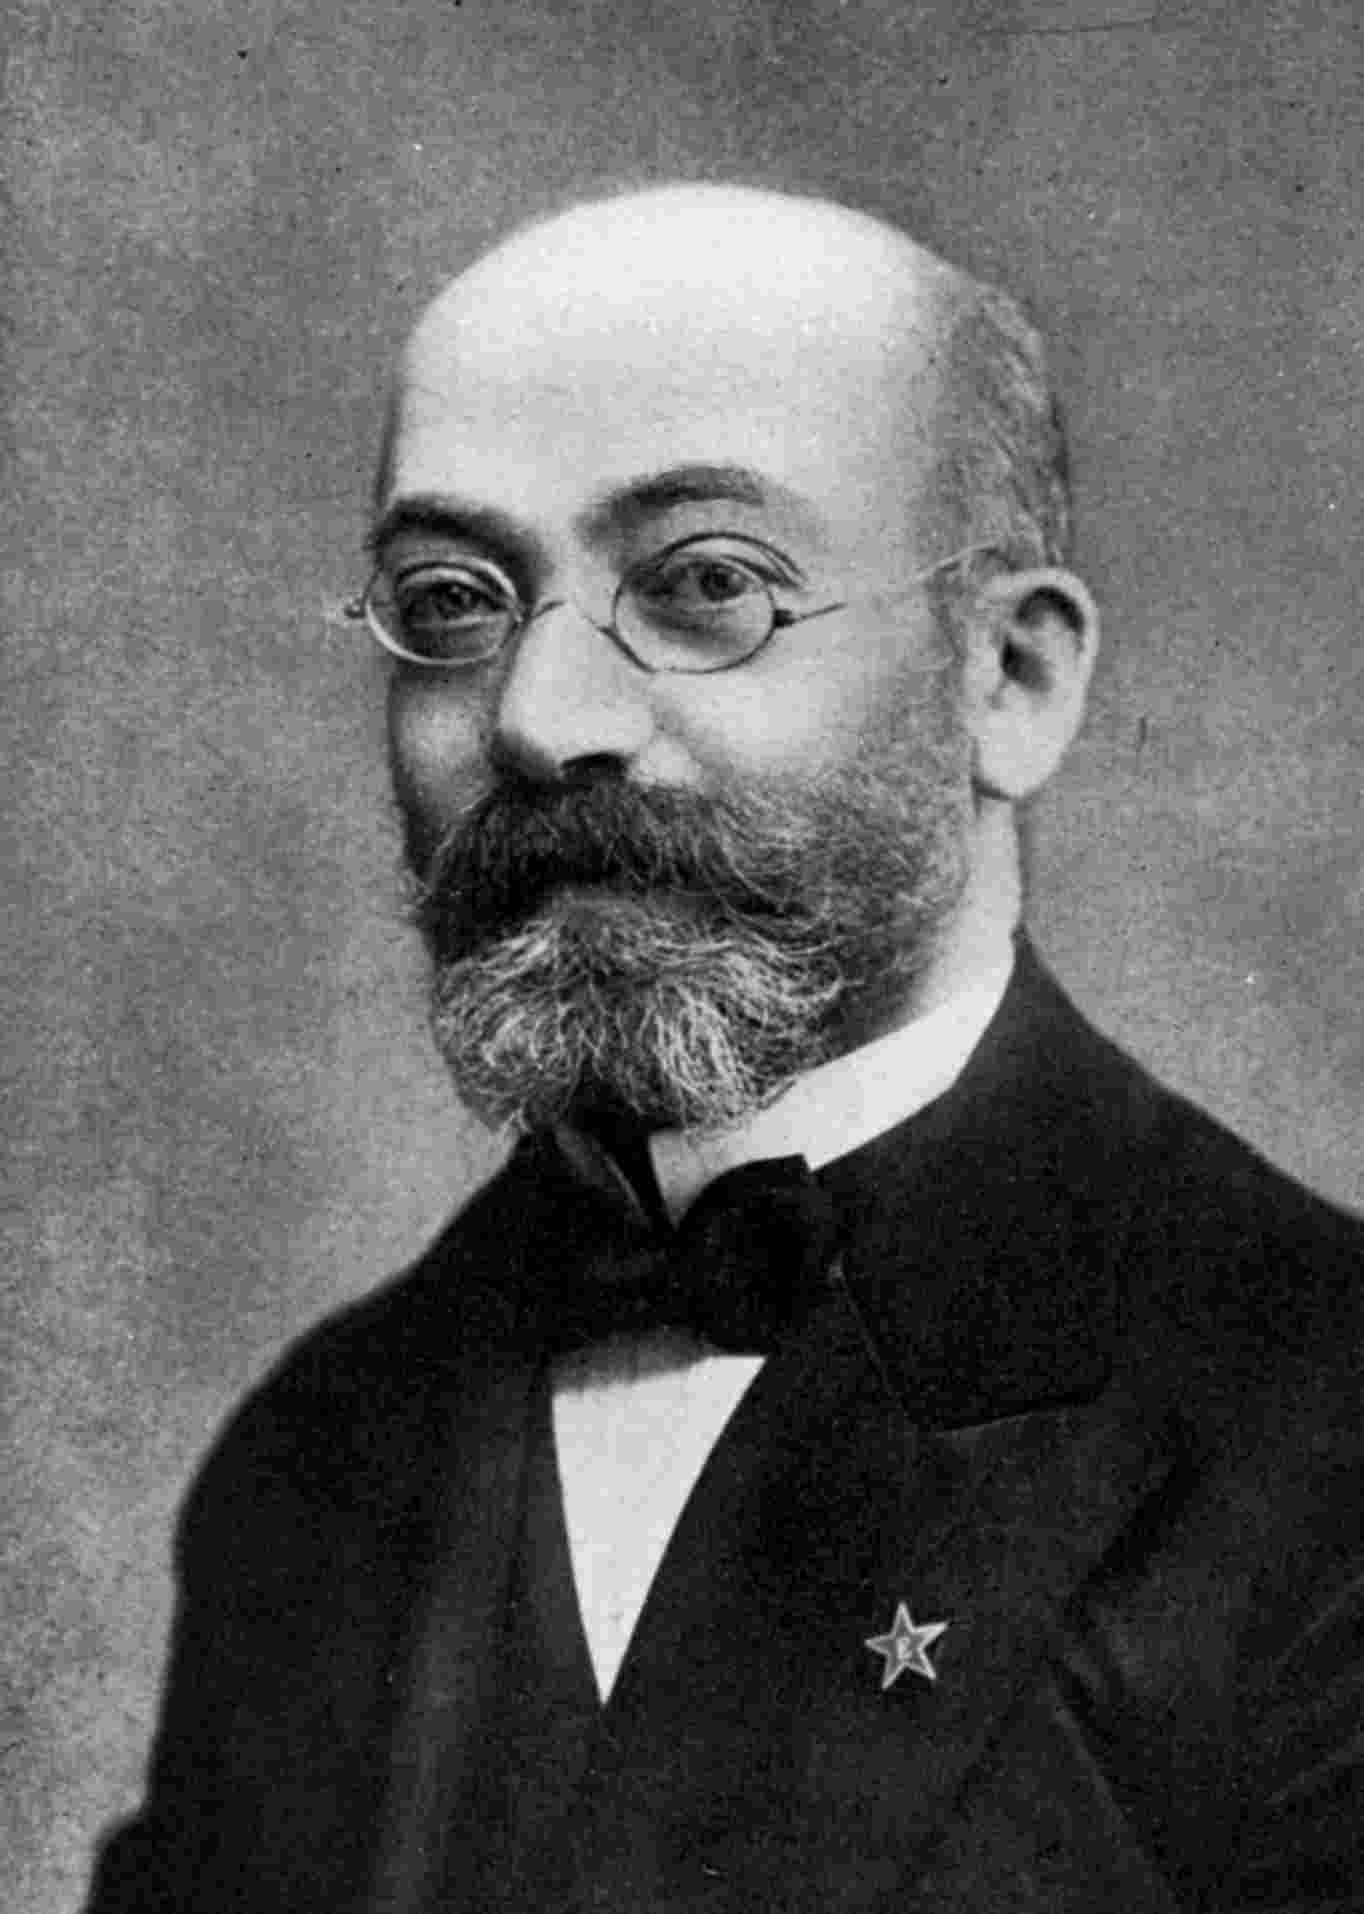
\includegraphics[scale=0.15]{../graphics/Zamenhof}
\end{figure}
\vspace*{0.5cm}
\nicefont
{\LARGE Lazaro Ludoviko ZAMENHOF} \\[1ex]
{\large Aŭtoro de la lingvo «Esperanto»} \\[1ex]
{\small (la 15-a de Decembro 1859 --- la 14-a de Aprilo 1917)}
 \vspace*{\stretch{1}}
\end{center}
\newpage
}

% Ligiloj, kaj ilia koloro 
%
\usepackage{color}
\definecolor{verda_ligilo}{rgb}{0,0.5,0}
\usepackage[colorlinks,linkcolor=verda_ligilo]{hyperref}
\usepackage{bookmark}

%
% Enkonduko speciala por Dua Libro
%

% need German-style quotes
% 
\usepackage{csquotes}
\MakeOuterQuote{"}
\setquotestyle{german}

% calculations
%
\usepackage{calc}

% tiparoj
%

% el dafont
\newfontfamily\latino{MkLatinoPlain}[LetterSpace=20]

% titlesec -- better section/chapter headings
%
% memoru:
% titleformat{command}[shape]{format}{label}{sep}{before-code}[after-code]
%
\renewcommand{\thesection}{\arabic{section}}
\titleformat{\section}[display]{\centering\large\bf}{}{0pt}{\scalebox{2}[1]}
\titlespacing{\section}{0pt}{1em}{1em}

% draws the "kajero" box on the title page
%
\newcommand{\kajerobox}{%
\begin{tikzpicture}[every node/.style={inner sep=0pt}]
\node[align=center](Text){\scalebox{0.5}[1]{\huge{\copper{KAJERO}} {\LARGE \textnumero} \copper 1.}};
\coordinate[shift={(-0.1cm,0.1cm)}](A) at (Text.north west);
\coordinate[shift={(0.1cm,0.1cm)}](B) at (Text.north east);
\coordinate[shift={(0.1cm,-0.1cm)}](C) at (Text.north east);
\coordinate[shift={(0.3cm,-0.1cm)}](D) at (Text.north east);
\coordinate[shift={(0.3cm,0.1cm)}](E) at (Text.south east);
\coordinate[shift={(0.1cm,0.1cm)}](F) at (Text.south east);
\coordinate[shift={(0.1cm,-0.1cm)}](G) at (Text.south east);
\coordinate[shift={(-0.1cm,-0.1cm)}](H) at (Text.south west);
\coordinate[shift={(-0.1cm,0.1cm)}](I) at (Text.south west);
\coordinate[shift={(-0.3cm,0.1cm)}](J) at (Text.south west);
\coordinate[shift={(-0.3cm,-0.1cm)}](K) at (Text.north west);
\coordinate[shift={(-0.1cm,-0.1cm)}](L) at (Text.north west);
\draw[very thick](A) -- (B) -- (C) -- (D) -- (E) -- (F) -- (G) -- (H) -- (I) -- (J) -- (K) -- (L) -- cycle;
\filldraw(A) circle [radius=1.25pt];
\filldraw(B) circle [radius=1.25pt];
\filldraw(D) circle [radius=1.25pt];
\filldraw(E) circle [radius=1.25pt];
\filldraw(G) circle [radius=1.25pt];
\filldraw(H) circle [radius=1.25pt];
\filldraw(J) circle [radius=1.25pt];
\filldraw(K) circle [radius=1.25pt];
\end{tikzpicture}}

% the command for the morpheme-separation stroke 
% differs from that in Unua Libro
%
\renewcommand{\,}{\raisebox{-1.1ex}{\relsize{-0.5}{\textquotesingle}}}


% Version number
%
\newcommand{\laversio}{0.96}

%
% End preamble and then begin title page
% 
\begin{document}
\sloppy
\begin{titlepage}

\newlength{\tempparskip}
\setlength{\tempparskip}{\parskip}
\setlength{\parskip}{2ex}

\vspace*{\fill}

\begin{center}

\scalebox{0.8}[1]{\latin\huge D\raisebox{0.6ex}{\underline{\small RO}} \so{ESPERANTO}.}

\pgfornament[width=0.3\textwidth]{83}\\[3ex]

\scalebox{1.3}[1.3]{\latino{\Huge{%
\scalebox{2}[2]{D}\thinspace{}\scalebox{1.3}[1]{UA}~%
\scalebox{2}[2]{L}\thinspace{}\thinspace{}\scalebox{1.3}[1]{IBRO}}}}\\[4ex]

\scalebox{1.5}[1]{\cowboyfont{\huge de~l’~lingvo}}\\[4ex]

\scalebox{2}{\shadowtext{\cowboyfont{\LARGE\spaceoutmed{INTERNACIA\thinspace}}}}

\pgfornament[width=0.5\textwidth]{82}\\[3ex]

\kajerobox

\pgfornament[width=0.2\textwidth]{85}

\scalebox{1}[0.5]{\LARGE Kosto 25 kopekoj.}

\pgfornament[width=0.2\textwidth]{86}\\[3ex]

\scalebox{0.7}[1]{\Large \spaceout{VARSOVIO.}}

\rule[1ex]{3em}{0.4pt}

\scalebox{1.5}[1]{{\large 1888.}}

\end{center}

\vspace*{\fill}

\setlength{\parskip}{\tempparskip}
\end{titlepage}

%
% Inside title page
%
\renewcommand{\footrulewidth}{0.4pt}
\setstretch{1.1}

\vspace*{12em}

\begin{table}[h]
\begin{center}
{\large Дозволено Цензурою. \\
\vspace{1ex}
Варшава, 18 Январа 1888 года.}
\end{center}

\end{table}

\setlength{\parskip}{0pt}

\vspace*{\fill}

\begin{flushright}
\begin{tabular}{r}
\hline
\bf\footnotesize Presejo de Ĥ. Kelter, Varsovio, strato Nowolipie N. 11.
\end{tabular}
\end{flushright}

\vspace*{\fill}

%
% Introduction
%
\titleformat{\chapter}[display]{\centering}{}{0pt}{\cowboyfont\LARGE}
\renewcommand{\footrulewidth}{0pt}
\chapter*{ANTAŬPAROLO.}
\addcontentsline{toc}{chapter}{Antaŭparolo}
\fancyhead[C]{--- \thepage{} ---}

\begin{center}
\pgfornament[width=0.3\textwidth]{88}
\end{center}

El\,ir\,ant\,e ankoraŭ unu foj\,o\,n antaŭ la estim\,at\,a publik\,o, mi sent\,as la dev\,o\,n antaŭ ĉio dank\,i la leg\,ant\,a\,n publik\,o\,n por la viv\,a kun\,sent\,o, kiu\,n ĝi montr\,is por mi\,a afer\,o. La mult\,a\,j promes\,o\,j, kiu\,j\,n mi ricev\,as, kaj el kiu\,j tre grand\,a part\,o est\,as sub\,skrib\,it\,a \glqq{}sen\,kondiĉ\,e\grqq{}, la leter\,o\,j kun kuraĝ\,ig\,o\,j aŭ konsil\,o\,j---ĉio tio ĉi montr\,as al mi, ke mi\,a profund\,a kred\,o je l' hom\,ar\,o mi\,n ne tromp\,is. La bon\,a geni\,o de l' hom\,ar\,o vek\,iĝ\,is: de ĉiu\,j flank\,o\,j al la labor\,o ĉiu\,hom\,a ven\,as amas\,o\,j, kiu\,j ordinar\,e est\,as tiel mal\,diligent\,a\,j por ĉia nov\,a afer\,o; jun\,a\,j kaj mal\,jun\,a\,j, vir\,o\,j kaj vir\,in\,o\,j---rapid\,as port\,i ili\,a\,n ŝton\,o\,n por la grand\,a, grav\,a kaj util\,eg\,a konstru\,o. Viv\,u l' hom\,ar\,o, viv\,u la frat\,ec\,o de l' popol\,o\,j, viv\,u etern\,e!

En mi\,a unu\,a verk\,o mi dir\,is, ke mi\,a\,n labor\,o\,n mi prezent\,as je l' temp\,o de unu jar\,o al la juĝ\,o de l' tut\,a mond\,o; kiam pas\,us la jar\,o, mi intenc\,is el\,don\,i libr\,et\,o\,n, en kiu est\,us analiz\,it\,a\,j ĉiu\,j pens\,o\,j esprim\,it\,a\,j de l' publik\,o, kaj uz\,int\,e tiu\,j\,n, kiu\,j efektiv\,e est\,us bon\,a\,j, mi don\,us al la lingv\,o la fin\,a\,n form\,o\,n, kaj post tio ĉi oni jam pov\,us komenc\,i la eldon\,o\,n de plen\,a\,j vort\,ar\,o\,j, libr\,o\,j, gazet\,o\,j kaj ceter\,e, ĉar tia\,n la lingv\,o jam est\,us tra\,ir\,int\,a la juĝ\,o\,n de l' tut\,a mond\,o, kaj ĉiu\,j plej grav\,a\,j mal\,bon\,aĵ\,o\,j, kiu\,j pov\,us est\,i trov\,it\,a\,j en ĝi, ĉar en verk\,o de unu hom\,o,---est\,us jam pli aŭ mal\,pli for\,ig\,it\,a\,j. Mi efektiv\,e intenc\,is silent\,i en la daŭr\,o de tut\,a jar\,o. Sed de l' tag\,o, kiam el\,ir\,is mi\,a libr\,et\,o, mi komenc\,is ricev\,i mult\,o\,n da leter\,o\,j kun demand\,o\,j kaj kun pet\,o\,j rapid\,ig\,i l' afer\,o\,n. Respond\,i je ĉiu leter\,o apart\,e est\,as por mi ne ebl\,e, kaj tial mi decid\,is respond\,i publik\,e je ĉiu\,j demand\,o\,j kaj propon\,o\,j, ĉar tiel unu respond\,o pov\,as serv\,i por mult\,a\,j demand\,ant\,o\,j. Ĉiu\,j respond\,o\,j far\,os unu libr\,o\,n, kiu prezent\,os daŭr\,ig\,o\,n de l' unu\,a libr\,o, kiu\,n mi el\,don\,is. Sed se mi vol\,us la respond\,o\,j\,n je ĉiu\,j demand\,o\,j el\,don\,i kun\,e, en unu libr\,o, mi dev\,us tro long\,e atend\,ig\,i mi\,a\,j\,n korespond\,ant\,o\,j\,n, dum tiu libr\,o est\,os pret\,a kaj el\,don\,it\,a,---tiom pli, ke konstant\,e al mi ven\,as nov\,a\,j demand\,o\,j; tial mi decid\,is el\,don\,i la libr\,o\,n kun la respond\,o\,j---per apart\,a\,j kajer\,o\,j, kiu\,j est\,os el\,las\,at\,a\,j en la daŭr\,o de la tut\,a jar\,o 1888 period\,e, kun inter\,temp\,o\,j de ĉirkaŭ du monat\,o\,j de unu kajer\,o ĝis la ven\,ont\,a. En tiu\,j ĉi kajer\,o\,j \emph{ĉiu\,j} demand\,o\,j est\,os respond\,it\,a\,j; je l' fin\,o de l' jar\,o 1888 el\,ir\,os la last\,a kajer\,o, kaj la \glqq{}Du\,a libr\,o de l' lingv\,o inter\,naci\,a\grqq{} est\,os fin\,it\,a.

Ankoraŭ unu afer\,o dev\,ig\,as mi\,n komenc\,i la el\,don\,o\,n de l' kajer\,o\,j, pri kiu\,j mi parol\,is: malgraŭ l' intenc\,o, kiu\,n mi esprim\,is en mia unu\,a verk\,o, komenc\,i la el\,don\,o\,n de libr\,o\,j ne pli fru\,e ol est\,os fin\,it\,a la juĝ\,o de l' publik\,o je l' lingv\,o propon\,it\,a de mi,---de ĉiu\,j flank\,o\,j ven\,as postul\,o\,j, ke mi kiom ebl\,e pli rapid\,e el\,don\,u ia\,n libr\,o\,n en la lingv\,o inter\,naci\,a, ke la publik\,o pov\,u kon\,iĝ\,i tiu\,n ĉi lingv\,o\,n ĉiu\,flank\,e, ĝi\,n el\,lern\,i pli rapid\,e kaj uz\,i ĝi\,n. La nombr\,o de tiu\,j ĉi postul\,o\,j est\,as tiel grand\,a, ke mi ne pov\,as jam aŭd\,i ili\,n silent\,e. El\,don\,ant\,e la \glqq{}Du\,a\,n libr\,o\,n de l' lingv\,o inter\,naci\,a\grqq{}, skrib\,it\,a\,n jam en tiu ĉi lingv\,o, mi don\,os al la dezir\,ant\,o\,j sufiĉ\,e da material\,o por leg\,i kaj la ebl\,o\,n tut\,e bon\,e el\,lern\,i la lingv\,o\,n; escept\,int\,e la tekst\,o\,n de l' libr\,o, kiu jam per si mem prezent\,os material\,o\,n por leg\,i, en la libr\,o est\,os ankaŭ pec\,o\,j sistem\,a\,j, por lern\,i kaj ripet\,i.

La tut\,a libr\,o hav\,os 5 --- 6 kajer\,o\,j\,n, en kiu\,j est\,os trov\,at\,a\,j respond\,o\,j je \emph{ĉiu\,j} demand\,o\,j, kiu\,j tuŝ\,as la lingv\,o\,n mem, ĝi\,a\,n konstru\,o\,n, ĝi\,a\,n est\,ont\,ec\,o\,n, kiel ĝi\,n bon\,e kaj fond\,e el\,lern\,i, kiel plej rapid\,e kaj plej cert\,e vast\,ig\,i ĝi\,a\,n uz\,o\,n en la mond\,o,---kaj ceter\,e. Kiam la last\,a kajer\,o de l' libr\,o est\,os el\,ir\,int\,a, tiam por la leg\,ant\,o neni\,o jam est\,os ne klar\,a: la societ\,o tiam kon\,os la tut\,a\,n anim\,o\,n de l' lingv\,o, ĝi tiam hav\,os \emph{plen\,a\,n} vort\,ar\,o\,n kaj pov\,os tut\,e \emph{liber\,e} uz\,i la lingv\,o\,n por \emph{ĉia\,j cel\,o\,j}, kiel ĝi pov\,as nun uz\,i ĉia\,n riĉ\,a\,n kaj pri\,labor\,it\,a\,n viv\,ant\,a\,n lingv\,o\,n. La de\,pend\,o de la lingv\,o de l' vol\,o aŭ de l' talent\,o de mi\,a propr\,a person\,o aŭ de ia ali\,a apart\,a person\,o aŭ person\,ar\,o---tut\,e for\,iĝ\,os. La lingv\,o tiam est\,os tut\,e pret\,a en ĉiu\,j plej mal\,grand\,a\,j ĝi\,a\,j part\,o\,j. La person\,o de l' aŭtor\,o tiam tut\,e for\,ir\,os de la scen\,o kaj est\,os forges\,it\,a. Ĉu mi post tio ankoraŭ viv\,os, ĉu mi mort\,os, ĉu mi konserv\,os la fort\,o\,n de mi\,a korp\,o kaj anim\,o, ĉu mi ĝi\,n perd\,os,---l' afer\,o tut\,e ne de\,pend\,os de tio, kiel la sort\,o de ia viv\,ant\,a lingv\,o tut\,e ne de\,pend\,as de l' sort\,o de tiu ĉi aŭ tiu person\,o.

Mult\,a\,j kred\,ebl\,e balanc\,as sen\,kred\,e la kap\,o\,n, leg\,ant\,e mi\,a\,j\,n vort\,o\,j\,n. Kiel tio est\,as ebl\,a, ili dir\,as, ke en la temp\,o de unu jar\,o la lingv\,o est\,us tut\,e kaj plen\,e pret\,a, tiel ke ĝi ne bezon\,us pli la labor\,o\,n de l' aŭtor\,o? Ke tiel grand\,eg\,a afer\,o, kiel la kre\,o kaj la en\,konduk\,o de lingv\,o tut\,mond\,a, en la temp\,o de unu jar\,o tiel matur\,iĝ\,us kaj fort\,iĝ\,us kaj ricev\,us tia\,n klar\,a\,n, ne\,ŝancel\,ebl\,a\,n ord\,o\,n, ke ĝi ne bezon\,us pli konduk\,ant\,o\,n! Sed mi esper\,as, ke jam post la du\,a aŭ la tri\,a kajer\,o la leg\,ant\,o vid\,os, ke mi ne fantazi\,as.

La leg\,ant\,o ne pens\,u, ke en la libr\,o, kiu\,n mi intenc\,as el\,don\,i, li vid\,os ia\,j\,n mir\,ind\,aĵ\,o\,j\,n. Tiu, kiu kutim\,is estim\,i la afer\,o\,j\,n ne laŭ ili\,a praktik\,a signif\,o kaj efektiv\,a ind\,o, sed laŭ la mir\,ind\,ec\,o kaj ne\,natur\,ec\,o de ili\,a nask\,o, est\,os kred\,ebl\,e tromp\,it\,a en si\,a\,j esper\,o\,j, kiam, leg\,ant\,e mi\,a\,n libr\,o\,n, li renkont\,os en ĝi sol\,e afer\,o\,j\,n simpl\,a\,j\,n kaj natur\,a\,j\,n. Sed la rezult\,at\,o\,j de tiu\,j ĉi simpl\,aĵ\,o\,j est\,os, kiel laŭ mi\,a esper\,o la leg\,ant\,o post\,e vid\,os kaj konfes\,os, ke post la fin\,o de l' jar\,o

\emph{a}) la lingv\,o est\,os fin\,it\,a kaj pret\,a tut\,e kaj plen\,e, tiom, ke ĝi tut\,e ne bezon\,os pli la labor\,o\,n de l' aŭtor\,o, kaj, kiel ĉiu el la viv\,ant\,a\,j lingv\,o\,j, ĝi far\,iĝ\,os tut\,e sen\,de\,pend\,a de ia apart\,a person\,o.

\emph{b}) la lingv\,o est\,os pli aŭ mal\,pli \emph{sen\,erar\,a}, ĉar ĝis tiu temp\,o ĝi jam est\,os tra\,ir\,int\,a la juĝ\,o\,n de l' tut\,a mond\,o, kaj ĉiu\,j mal\,bon\,aĵ\,o\,j, kiu\,j pov\,us est\,i trov\,it\,a\,j en tiu ĉi labor\,o de \emph{unu person\,o}, est\,os for\,ig\,it\,a\,j per la konsil\,o\,j de l' tut\,a mond\,o kun\,e.

Leg\,ant\,e la unu\,a\,j\,n kajer\,o\,j\,n de mi\,a libr\,o, mult\,a\,j kred\,ebl\,e rest\,os ne kontent\,a\,j, ĉar ili ebl\,e tie ne trov\,os respond\,o\,j\,n je l' demand\,o\,j, kiu\,j\,n \emph{ili} send\,is; kaj ĉar li\,a \emph{propr\,a} demand\,o en la okul\,o\,j de ĉiu est\,as la plej grav\,a, mult\,a\,j kred\,ebl\,e ek\,kri\,os: \glqq{}Kio li parol\,as sol\,e pri afer\,o\,j tut\,e sen\,signif\,a\,j, kaj pri l' afer\,o\,j efektiv\,e grav\,a\,j li ne parol\,as eĉ unu vort\,o\,n!\grqq{} La leg\,ant\,o ofer\,u al mi iom da atend\,em\,o, ĉar ĝis la fin\,o de l' jar\,o \emph{ĉiu\,j} est\,os kontent\,ig\,it\,a\,j. Se en unu de l' unu\,a\,j kajer\,o\,j tiu aŭ ali\,a demand\,o est\,os jam ŝajn\,e fin\,it\,a kaj liber\,ig\,os la lok\,o\,n por ali\,a demand\,o, tio tut\,e ne dev\,as pens\,ig\,i, ke mi jam pli ne parol\,os pri ĝi. Ĉar pri mult\,a\,j demand\,o\,j mi don\,os en la unu\,a\,j kajer\,o\,j sol\,e mi\,a\,n \emph{person\,a\,n} juĝ\,o\,n, sed post\,e mi re\,ven\,os al ili kaj don\,os la decid\,o\,n \emph{fin\,a\,n}, ricev\,it\,a\,n per la juĝ\,o de l' \emph{publik\,o}.

Pro la cel\,o\,j de l' afer\,o la libr\,o ne est\,os unu sistem\,a verk\,o---ĝi est\,os simpl\,e mi\,a inter\,parol\,o kun l' amik\,o\,j de l' lingv\,o inter\,naci\,a.

La kost\,o de ĉiu kajer\,o est\,os 25 kopek\,o\,j. Kiu vol\,as, ke mi send\,u al li ĉiu\,n ven\,ont\,a\,n kajer\,o\,n tuj, kiam ĝi est\,os pret\,a kaj el\,ir\,os el la pres\,ej\,o, tiu send\,u al mi la kost\,o\,n de l' ven\,ont\,a kajer\,o tuj post la ricev\,o de l' antaŭ\,ir\,ant\,a.

\begin{center}
\rule{0.2\textwidth}{0.4pt}
\end{center}

Antaŭ\,e ol fin\,i la antaŭ\,parol\,o\,n, mi permes\,as al mi ripet\,i ankoraŭ la pet\,o\,n, kiu\,n mi jam esprim\,is en mi\,a unu\,a verk\,o: ĉiu pen\,e juĝ\,u la afer\,o\,n, propon\,it\,a\,n de mi, kaj ĉiu montr\,u al mi la erar\,o\,j\,n, kiu\,j\,n li trov\,is en ĝi, aŭ la pli\,bon\,ig\,o\,j\,n, kiu\,j\,n li pov\,as propon\,i. Se la leg\,ant\,o ne pov\,is ankoraŭ tut\,e bon\,e ek\,kon\,i mi\,a\,n afer\,o\,n el mi\,a unu\,a libr\,et\,o, tiu ĉi mi\,a du\,a libr\,o pov\,ig\,os li\,n post kelk\,a temp\,o ek\,kon\,i ĝi\,n tut\,e kaj ĉiu\,flank\,e. Ke mi\,a afer\,o ven\,u al dezir\,inda\, cel\,o, est\,as neces\,e ne sol\,e, ke la mond\,o dir\,u si\,a\,n juĝ\,o\,n pri tiu ĉi afer\,o, sed ke mi sci\,u la juĝ\,o\,n de l' mond\,o kaj pov\,u ĝi\,n uzi por mi\,a labor\,o.

Dis\,send\,ant\,e mi\,a\,n unu\,a\,n verk\,o\,n al la redakci\,o\,j de l' gazet\,o\,j, mi pet\,is ili\,n al\,send\,i al mi tiu\,n numer\,o\,n de l' gazet\,o, en kiu est\,os kritik\,o de mi\,a afer\,o; sed bedaŭr\,ind\,e tre mal\,mult\,a\,j plen\,um\,is mi\,a\,n pet\,o\,n, kaj sci\,iĝ\,i mem, kie, kiam kaj kio est\,is parol\,at\,a pri mi\,a afer\,o, est\,as por mi tut\,e ne ebl\,a. Tial mi pet\,as la \emph{leg\,ant\,o\,j\,n} de l' gazet\,o\,j send\,i al mi la numer\,o\,j\,n, en kiu\,j ili leg\,is io\,n pri l' afer\,o, propon\,it\,a de mi, kaj jam antaŭ\,e mi esprim\,as al ili mi\,a\,n kor\,a\,n dank\,o\,n. Mi pet\,as ĝi\,n ne por \emph{mi}, sed pro l' \emph{afer\,o}.

Fin\,e, antaŭ la komenc\,o de mi\,a inter\,parol\,o kun la amik\,o\,j de l' lingv\,o inter\,naci\,a, mi esprim\,as ankoraŭ unu foj\,o\,n mi\,a\,n varm\,eg\,a\,n dank\,o\,n al la publik\,o por la help\,em\,o, kiu\,n ĝi montr\,is al mi; mi esper\,as, ke la kun\,sent\,o de l' publik\,o ne mal\,varm\,iĝ\,os, sed konstant\,e kaj sen\,ĉes\,e kresk\,os, kaj post tre mal\,long\,a temp\,o ven\,os al cel\,o la afer\,o, je kiu labor\,as ĉiu\,j sfer\,o\,j de l' hom\,a societ\,o. 

\begin{center}
\pgfornament[width=0.3\textwidth]{83}\\[12pt]
\phantomsection
\addcontentsline{toc}{chapter}{I.}
\scalebox{2}[1]{\large\cowboyfont{I.}}
\end{center}

Antaŭ ĉio mi parolos kelkajn vortojn pri tiuj kritikoj, kiujn mi ĝis hodiaŭ aŭdis aŭ legis, en gazetoj aŭ en leteroj al mi, kvankam mi devas antaŭsciigi la leganton, ke tiu ĉi punkto estas en miaj okuloj tre grava kaj poste mi ankoraŭ parolos pri ĝi pli vaste. Mi ne volus fari ian\footnote{\emph{Komento el kompostanto:} Ne klaras ĉi tie, ĉu Zamenhofo intencis la modernan "iam" aŭ la modernan "ian".  Ĉu li \emph{neniam} volus fari premon?  Aŭ ĉu li volus \emph{nenian} premon?  Ĉar ne klaras, mi forlasas la originalan "ian" ĉi tie.} premon sur la juĝo de l' publiko, kaj mi volus, ke la mondo kreu mem sian decidon en la afero, kiun mi proponis. Sed kelkaj kritikoj estis tiel skribitaj, ke mi ne povas tute silenti pri ili.

\emph{a}) Unuj parolis pri l' aŭtoro, anstataŭ paroli pri l' afero. Ili aŭ ŝutis komplimentojn al la aŭtoro, rigardigis, kiom da malfacila laboro kredeble la afero min kostis, kaj, laŭdante la \emph{aŭtoron}, ili preskaŭ tute forgesis paroli pri l' utileco kaj la signifo de l' \emph{afero} kaj decidigi la publikon labori por ĝi; aliaj, ne trovante en mia verko la instruitan miksaĵon kaj la instruita-teorian filozofadon, kiujn ili kutimis renkonti en ĉia grava verko, timis, ke la pseŭdonima aŭtoro eble estas ne sufiĉe instruita aŭ ne sufiĉe merita, kaj ili timis esprimi decidan juĝon, pli multe penante malkovri, kiu estas la pseŭdonima aŭtoro. Por igi la kritikistojn tute apartigi la \emph{aferon} de la \emph{aŭtoro}, mi publike diras mem, ke mi ne estas multege instruita lingvisto, ke mi estas tute senmerita kaj ne konata en la mondo. Mi scias, ke mia konfeso malvarmigos multajn por la afero, sed mi volas, ke oni juĝu ne l' aŭtoron, sed la verkon. Se la verko estas bona, prenu ĝin; se ĝi estas malbona---ĵetu ĝin. Per kia vojo mi venis al la kreo de mia lingvo kaj laŭ kiaj metodoj mi laboris,---mi ankoraŭ parolos, sed en unu de la \emph{venontaj} kajeroj; ĉar laŭ mi tiu ĉi demando estas por la publiko sen signifo: por la mondo estas gravaj sole la \emph{rezultatoj}.

\emph{b}) Aliaj ekbrilis per senfinaj filozofadoj kaj skribis instruitajn artikulojn, tute ne pensinte kaj ne demandinte sin, ĉu ili parolas logike kaj afertuŝante. Anstataŭ provi praktike (kion fari estas tre facile), ĉu la lingvo, proponita de mi, taŭgas por internacia kompreniĝo, ĉu ĝi efektive al ĉiu donas la eblon esti komprenata de personoj alinaciaj,---ili parolis pri la fiziologio kaj historio de l' lingvoj vivaj; anstataŭ provi per ilia propra orelo, ĉu mia lingvo estas bonsona aŭ ne,---ili teorie parolis pri leĝoj de bonsoneco; anstataŭ analizi, ĉu mi bone kreis la vortaron kaj ĉu oni ne povus fari ĝin ankoraŭ pli komprenebla kaj pli praktika, ili diris, ke la vortaro devas esti farita el radikoj Sanskritaj aŭ el vortoj, prenitaj mikse el ĉiuj lingvoj de l' mondo. (La lingvo multe per tio ĉi \emph{perdus}, fariĝinte tute ne komprenebla; sed kion ĝi \emph{gajnus}, esceptinte la sennecesan instruitan eksteron? tion ĉi ili tute forgesis sin demandi.)

\emph{c}) Aliaj skribis kritikon pri mia afero, eĉ ne leginte bone mian malgrandan broŝuron kaj eĉ ne peninte kompreni la aferon. Tiel ekzemple la unuatempajn signetojn inter la partoj de l' vortoj ili tute ne komprenis, kaj skribante ekzemple \emph{\glqq{}ensong, oprinc, in, o, nmivid, is\grqq{}} (anstataŭ: \emph{\glqq{}en sonĝ\,o princ\,in\,o\,n mi vid\,is\grqq{}}), ili rigardigis iliajn legantojn, \glqq{}kiel malbonsona kaj nekomprenebla la lingvo estas\grqq{}! La projekton de l' tutmonda voĉdono, kiu kun la efektiva kaj senkondiĉa signifo de l' lingvo tute ne estas kunligita, kaj kiu estas proponita sole por tio, ke la lingvo pli rapide el \emph{internacia} fariĝu \emph{tutmonda},---ili prenis por la plej grava kaj fonda parto de l' afero kaj komprenigis la legantojn, ke \glqq{}ĉar dek milionoj adeptoj (!) neniam estos kolektitaj, tial la afero tute ne havas estontecon\grqq{}! Kelkajn fojojn mi eĉ legis longajn artikulojn pri mia afero, kie estis videble, ke la aŭtoroj eĉ ne vidis mian verkon.

\emph{ĉ}) Aliaj, anstataŭ paroli pri la utileco aŭ la senutileco de mia lingvo, donis sole sensencajn ŝercojn, kiuj de iliaj legantoj estis eble prenataj por kritiko, ĉar multaj legantoj propran juĝon ne havas, kaj la plej malsaĝaj ŝercoj je ia afero estas por ili sufiĉa vidigo, ke la afero estas \glqq{}ridinda\grqq{} kaj taŭgas por nenio.

Mi ne deziras laŭdon, mi volas, ke oni min helpu forigi la erarojn, kiujn mi faris, kaj ju la kritikoj de mia lingvo estas pli severaj, des pli danke mi ilin alprenas, se ili nur havas la celon montri al mi la erarojn de mia afero, ke mi ilin bonigu, sed ne ridi sen senco aŭ insulti sen kaŭzo. Mi scias tre bone, ke la verko de \emph{unu homo} ne povas esti senerara, se tiu homo eĉ estus la plej genia kaj multe pli instruita ol mi. Tial mi ne donis ankoraŭ al mia lingvo la finan formon; mi ne parolas: \glqq{}jen la lingvo estas kreita kaj preta, tiel mi volas, tia ĝi estu kaj tia ĝi restu!\grqq{} Ĉio bonigebla estos bonigata per la konsiloj de l' mondo. Mi ne volas esti \emph{kreinto} de l' lingvo, mi volas nur esti \emph{iniciatoro}. Tio ĉi estu ankaŭ respondo al tiuj amikoj de l' lingvo internacia, kiuj estas neatendemaj kaj volus jam vidi librojn kaj gazetojn en la lingvo internacia, plenajn vortarojn, vortarojn nacia-internaciajn kaj cetere. Ne malfacile estus por mi kontentigi tiujn ĉi amikojn; sed ili ne forgesu, ke tio ĉi estus danĝera por la afero mem, kiu estas tiel grava, ke estus nepardoneble faradi laŭ la propra decido de unu homo. Mi ne povas diri, ke la lingvo estas preta, ĝis ĝi estos trairinta la juĝon de l' publiko. Unu jaro ne estas eterno, kaj tamen tiu ĉi jaro estas tre grava por l' afero. Tiel ankaŭ mi ne povas fari iajn ŝanĝojn en la lingvo tuj post la ricevo de la konsiloj, se tiuj ĉi konsiloj eĉ estus la plej seneraraj kaj venus de la plej kompetentaj personoj. En la daŭro de la tuta jaro 1888 la lingvo restos \emph{tute sen ŝanĝo}; sed kiam la jaro estos finita, tiam ĉiuj necesaj ŝanĝoj, antaŭe analizitaj kaj provitaj, estos publikigitaj, la lingvo ricevos la finan formon, kaj tiam komencos ĝia plena funkciado. Juĝante laŭ la konsiloj, kiuj estas senditaj al mi ĝis hodiaŭ, mi pensas, ke la lingvo kredeble estos ŝanĝita tre malmulte, ĉar la plej granda parto de tiuj konsiloj estas ne praktika kaj kaŭzita de ne sufiĉa pripensado kaj provado de l' afero; sed diri, ke la lingvo tute ne estos ŝanĝita, mi tamen ne povas. Cetere, ĉiuj proponoj, kiujn mi ricevas, kune kun mia juĝo pri ili, estos prezentataj al la juĝo de l' publiko aŭ de ia el la jam konataj instruitaj akademioj, se inter tiuj ĉi estos trovita unu, kiu volos preni tiun ĉi laboron. Se ia kompetenta akademio min sciigos, ke ĝi volas preni tiun ĉi laboron, mi tuj sendos al ĝi la tutan materialon, kiu estas ĉe mi, mi fordonos al ĝi la tutan aferon, mi foriros kun la plej granda ĝojo je eterne de l' sceno, kaj el aŭtoro kaj iniciatoro mi fariĝos simpla amiko de l' lingvo internacia, kiel ĉiu alia amiko. Se tamen nenia el la instruitaj akademioj volos preni mian aferon, tiam mi daŭrigos la publikigadon de l' proponoj, sendataj al mi, kaj laŭ mia propra pensado kaj laŭ la pensoj de l' publiko, sendataj al mi pri tiuj proponoj, mi mem antaŭ la fino de l' jaro decidos la finan formon de l' lingvo kaj mi sciigos, ke la lingvo estas preta. 

\begin{center}
\phantomsection
\scalebox{2}[1]{\large\cowboyfont II.}
\addcontentsline{toc}{chapter}{II.}
\end{center}

La nombro 10,000,000, pri kiu estas parolita en mia unua verko, ŝajnas al multaj absolute ne ricevebla. La plej granda parto de l' mondo efektive kredeble estos tiel senmova, ke ĝi de si mem ne donos voĉon, malgraŭ ke la afero estas tiel grava kaj la laboro de l' voĉdono tiel malgrandega. Sed se l' amikoj de l' lingvo internacia, anstataŭ timegi la nombron, laboros por la afero kaj kolektos tiom voĉojn, kiom ili povos, tiam la necesa nombro da voĉoj povas esti ricevita en la plej mallonga tempo.

Kiam mi proponis la voĉdonon, mi profunde kredis, ke pli frue aŭ pli malfrue 10,000,000 voĉoj estos kolektitaj. La rezultatoj, kiuj sin montris ĝis hodiaŭ, ankoraŭ plifortigas mian kredon. Sed ni prenu, ke mi fantazias, ke mi eraras, ke mi tro multe esperas,---ke sur la tuta tero ne estos kolektita eĉ unu miliono da voĉoj \ldots{} kion l' afero tiam perdos? Kelkaj konsilas al mi, ke mi forĵetu la voĉdonon aŭ ke mi malgrandigu la nombron da postulataj voĉoj ĝis unu miliono; \glqq{}ĉar\grqq{}, ili diras, \glqq{}danke la fantazian punkton de l' voĉdono, afero per si mem tiel utila, povas fari fiaskon.\grqq{} Sed kie, sinjoroj, vi prenis, ke la veno al celo de l' afero dependas de l' rezultatoj de la voĉdono? Tiuj, kiuj trovas, ke mia lingvo estas inda je lerno, sendas al mi promesojn senkondiĉajn kaj lernas la lingvon sen ia atendo. Sendepende de l' iro de la voĉdono en tiu ĉi lingvo estos eldonataj libroj kaj gazetoj, kaj la afero sin movos antaŭen. La voĉdonon mi proponis sole por tio, ke al la afero povu esti altiritaj per \emph{unu fojo} tutaj \emph{amasoj} da homoj, ĉar mi scias, ke preni ian laboron, eĉ la plej malgrandan, ne ĉiu konsentos, sed helpi aferon tre utilan, kie estas postulata nek laboro, nek mono,---ne multaj malkonsentos, tiom pli, se troviĝos memorigantoj. Mi ripetas: profunde mi kredas, ke pli frue aŭ pli malfrue 10,000,000 voĉoj estos kolektitaj, kaj tiel je unu bela tago ni sciiĝos, ke la lingvo internacia fariĝis tutmonda; sed se eĉ la nombro de l' voĉoj neniam venus al dek milionoj,---la afero pro tio ĉi tute ne estos perdita.

Kelkaj provis montri al mi, ke mia projekto de l' voĉdono estas \emph{matematike} ne ebla; tiel ekzemple unu faris jenan kalkulon: \glqq{}se ni prenos, ke la enskribado de ĉiu promesanto okupos ne pli multe ol unu minuton, kaj vi, forĵetinte ĉian alian laboron, vin okupos sole je tiu ĉi afero, laborante sen ripozo 15 horojn ĉiutage,---tiam la pretigo de la libro de l' voĉoj okupos 30 jarojn, kaj por eldoni ĝin vi bezonos la riĉecon de Krezo!\grqq{} La kalkulo ŝajne estas tute prava kaj povas timigi ĉiun,---tamen se la skribinto de tiu ĉi kalkulo bone pensus pri ĝi, li tre facile ekvidus, ke tie ĉi estas sofismo, kaj se nur efektive estos alsenditaj dek milionoj promesoj, la libron de l' voĉdono oni povos pretigi kaj eldoni en kelkaj monatoj kaj sen iaj riĉecoj de Krezo. Ĉar kiu diras, ke la tuta libro devas esti propramane skribita de unu persono? Ke ĉe ĉiu pli granda afero estas uzata \emph{divido de laboro}, la skribinto tute forgesis! Tiaj \glqq{}timigaj\grqq{} libroj estas eldonataj ĉiutage en granda nombro, kaj tio ne sole ne estas neebla, sed neniu eĉ en tio vidas ion grandegan, mirindan. Se vi kolektos la numerojn de ia ĉiutaga gazeto por unu jaro, vi ricevos libron, kiu laŭ grandeco kaj kosto egalas la elirontan libron de l' voĉoj, kaj laŭ la malfacileco de l' pretigo multe superas mian libron, de kiu la pretigo estas laboro pure meĥanika. Tiel ĉiujare en la mondo estas eldonataj miloj kaj dekmiloj da tiaj \glqq{}neeblaj\grqq{} libroj, kaj tamen neniu el la redaktoroj estas mirindaĵisto. Sinjoroj la kalkulantoj forgesis tiun simplan leĝon, kiun ili povas vidi sur ĉiu paŝo, ke tio, kio ĉe unu homo postulas 30 jarojn, ĉe cent homoj okupos sole 4 monatojn, kaj tio, kio estas neebla por unu persono, estas ludilo por grupo da personoj.

Al ĉiuj amikoj de l' lingvo internacia mi ripetas ankoraŭ mian peton: ne forgesu la promesojn kaj kolektu ilin kie kaj kiom vi povas. Multaj pensas, ke ili ne devas sendi promeson, ĉar \glqq{}la aŭtoro eĉ scias, ke ili ellernos aŭ jam ellernis la lingvon\grqq{}! Sed la promeso estas necesa ne por mi, sed por la statistiko. Se iu eĉ skribis al mi kelkajn leterojn en la lingvo internacia, mi ne povas lin nomi internaciisto, ĝis li ne sendis al mi sian promeson. Ne diru, ke de unu aŭ kelkaj promesoj la grandega nombro ne pleniĝos: ĉiu maro estas kreita de apartaj gutoj, kaj la plej granda nombro devas kaj povas esti ricevita el apartaj unuoj. Memoru, ke se eĉ la esperata nombro estas ne ricevota, vi nenion perdas, sendante la promeson. 

\begin{center}
\phantomsection
\scalebox{2}[1]{\large\cowboyfont{III.}}
\addcontentsline{toc}{chapter}{III.}
\end{center}

La venontajn apartajn pecojn mi donas, ke la lernantoj povu ripeti praktike la regulojn de l' gramatiko internacia kaj kompreni bone la signifon kaj la uzon de l' sufiksoj kaj prefiksoj.


\mysect{1.}

Amik\,o ven\,is (= unu el la amik\,o\,j ven\,is).---La amik\,o ven\,is (= la kon\,at\,a amik\,o, aŭ la amik\,o, kiu\,n oni atend\,is).---Don\,u al mi libr\,o\,n.---Don\,u al mi la libr\,o\,n, kiu\,n vi promes\,is al mi.---Tiu ĉi ĝarden\,o est\,as am\,at\,a lok\,o de bird\,o\,j.---La fenestr\,o est\,as am\,at\,a lok\,o de la bird\,o\,j (= ni\,a\,j bird\,o\,j).---La vort\,o "la" est\,as nom\,at\,a "artikul\,o"; ĝi estas uz\,at\,a tiam, kiam ni parol\,as pri objekt\,o\,j kon\,at\,a\,j. Anstataŭ "la" oni pov\,as ankaŭ dir\,i "l' ", se ĝi ne est\,os mal\,bon\,son\,e.---Se iu ne kompren\,as bon\,e la uz\,o\,n de la artikul\,o, li pov\,as \emph{tut\,e ĝi\,n ne uz\,i}, ĉar ĝi est\,as oportun\,a sed ne neces\,a. 


\mysect{2.}

Jen est\,as la patr\,o.---Mi aŭd\,as la voĉ\,o\,n de la patr\,o.---Mi ricev\,is donac\,o\,n de la patr\,o.---Dir\,u al la patr\,o, ke mi est\,as san\,a.---Ni ir\,os al la patr\,o.---Karol\,o aĉet\,is por si\,a kuz\,in\,o horloĝ\,et\,o\,n kun tri montr\,ant\,o\,j.---Ni vid\,as per la okul\,o\,j.---Rakont\,u al ni la nov\,aĵ\,o\,j\,n, kiu\,j\,n vi aŭd\,is pri ni\,a\,j mal\,feliĉ\,a\,j frat\,o\,j.---De kiu vi ĝi\,n aŭd\,is?---Mi pens\,as pri la sort\,o de mi\,a frat\,in\,o, kaj mi kalkul\,as jam la minut\,o\,j\,n ĝis ni\,a re\,vid\,o.---Aŭgust\,o est\,as bon\,a, Mari\,o est\,as pli bon\,a ol Aŭgust\,o, sed Ernest\,in\,o est\,as la plej bon\,a el ĉiu\,j mi\,a\,j ge\,frat\,o\,j.---La mal\,grand\,a\,n fil\,in\,o\,n de mi\,a najbar\,o mi am\,as ne mal\,pli ol mi\,a\,n propr\,a\,n infan\,o\,n; hodiaŭ mi aĉet\,is por ŝi tre bel\,a\,n lud\,il\,o\,n. 


\mysect{3.}

Ses\,dek minut\,o\,j far\,as unu hor\,o\,n, kaj du\,dek kvar hor\,o\,j far\,as unu plen\,tag\,o\,n.---Mi loĝ\,as en la tri\,a etaĝ\,o.---Hodiaŭ est\,as la dek kvin\,a (tag\,o) de April\,o.---La du\,dek\,a de Februar\,o est\,as la kvin\,dek unu\,a tag\,o de l' jar\,o.---Tiu ĉi river\,o hav\,as du\,cent naŭ\,dek kvar kilometr\,o\,j\,n da long\,o.---Georg\,o Vaŝington\,o est\,is nask\,it\,a la du\,dek du\,a\,n Februar\,o\,n (aŭ: je l' du\,dek du\,a Februar\,o) de l' jar\,o mil sep\,cent tri\,dek dua.---Send\,u al mi prunt\,e dek\,du\,o\,n da fork\,et\,o\,j.---Tio ĉi okaz\,is antaŭ cent jar\,o\,j.---Mi aĉet\,is du ŝrank\,o\,j\,n kaj pag\,is por ili cent frank\,o\,j\,n.---Jen estas cent\,o da pom\,o\,j.---En tiu ĉi land\,o loĝ\,as tri milion\,o\,j krist\,an\,o\,j (aŭ: da krist\,an\,o\,j).---Du\,obl\,a faden\,o est\,as pli fort\,a ol unu\,obl\,a.---De tiu tag\,o mi\,a amik\,ec\,o al li du\,obl\,iĝ\,is.---Kvar\,obl\,e kvin est\,as du\,dek.---Kvar foj\,o\,j\,n mi jam est\,is tie.---Du\,on\,o\,n de tiu ĉi pir\,o mi manĝ\,is, kvar\,on\,o\,n mi don\,is al mi\,a nev\,o, kaj la last\,a\,n kvar\,on\,o\,n mi for\,ĵet\,is.---Du\,dek unu est\,as tri sep\,on\,o\,j de kvar\,dek naŭ.---Kvin\,op\,e ili tir\,is la kest\,o\,n kaj tamen ne pov\,is ĝi\,n alt\,ir\,i al la dom\,o.---Se vi ven\,os al li tri\,op\,e, li re\,don\,os, kio\,n li pren\,is; ĉar unu\,e li tim\,os vi\,a\,n fort\,o\,n, kaj du\,e li ne pov\,os si\,n prav\,ig\,i.---Al ĉiu el la labor\,ant\,o\,j li don\,is po kvin dolar\,o\,j\,n. 


\mysect{4.}

Mi vi\,n ne kompren\,as, sinjor\,o.---Vi est\,as tre obstin\,a, mi\,a amik\,o.---Vi ĉiu\,j est\,as tro fier\,a\,j.---"Vi" ni dir\,as egal\,e al unu person\,o aŭ objekt\,o kaj al mult\,a\,j; tio ĉi est\,as far\,it\,a pro oportun\,ec\,o, ĉar, parol\,ant\,e kun iu, ni oft\,e ne sci\,as, kiel dir\,i al li: "vi" aŭ "ci" ("ci" signif\,as la du\,a\,n person\,o\,n de l' unu\,nombr\,o; sed tiu ĉi vort\,o est\,as trov\,at\,a sol\,e en la plen\,a vort\,ar\,o; en la lingv\,o mem ĝi preskaŭ neniam est\,as uz\,at\,a).---La ĉap\,ist\,o ne ven\,os, ĉar li est\,as mal\,san\,a; se ven\,os li\,a edz\,in\,o, don\,u al ŝi mi\,a\,n ĉapel\,o\,n; se ven\,os li\,a plej mal\,juna fil\,o, vi pov\,as ankaŭ ĝi\,n don\,i al li; sed se ven\,os li\,a mal\,grand\,a infan\,o, don\,u al ĝi nenio\,n.---Jen est\,as la hund\,o, don\,u al ĝi ost\,o\,n, kaj vok\,u la kat\,in\,o\,n, ĝi ricev\,os pec\,o\,n da viand\,o.---Mi am\,as mi\,n, ĉar ĉiu am\,as si\,n mem.---Vi estim\,as vi\,n mem, sed ali\,a\,j vi\,n ne estim\,as; mi\,a frat\,o estim\,as si\,n ne mult\,e, sed ali\,a\,j li\,n tre estim\,as.---Montr\,u al mi vi\,a\,n kalkul\,o\,n.---Ili konduk\,is la koleg\,o\,j\,n en si\,a\,n loĝ\,ej\,o\,n, anstataŭ ir\,i kun ili en ili\,a\,n.---Oni dir\,as, ke vi est\,as riĉ\,a. 


\mysect{5.}

 Kial vi ne respond\,as al mi, kiam mi vi\,n demand\,as?---La patr\,o skrib\,as leter\,o\,n, kaj la infan\,o\,j prepar\,as si\,a\,j\,n lecion\,o\,j\,n.---Kio\,n li babil\,as?---Li babil\,ad\,as la tut\,a\,n tag\,o\,n.---Ni\,a gast\,o kant\,is la ĉiu\,kon\,at\,a\,n romanc\,o\,n de N.---Mi\,a onkl\,o ek\,kant\,is kaj tuj ĉes\,is, sed mi\,a frat\,o kant\,ad\,is la tut\,a\,n vesper\,o\,n.---Karol\,in\,o ĉiam obe\,ad\,is la ordon\,o\,j\,n de si\,a patr\,in\,o, sed hodiaŭ ŝi ne obe\,is.---Kiam mi ven\,is al li, li tuj fin\,is si\,a\,n labor\,o\,n.---Kiam mi ven\,is al li, li fin\,ad\,is si\,a\,n labor\,o\,n.---Vi ne mal\,help\,is mi\,n, ĉar kiam vi ven\,is, mi est\,is jam fin\,it\,a mi\,a\,n labor\,o\,n.---Li batal\,os, ĉar li ne dorm\,os trankvil\,e, ĝis li est\,os venk\,int\,a la mal\,amik\,o\,n.---Se mi nur est\,us san\,a, mi est\,us tut\,e kontent\,a.---Se ili est\,us dir\,int\,a\,j la ver\,o\,n, ili ne est\,us nun pun\,at\,a\,j; nun ili konfes\,is ĉio\,n, sed ĝi est\,is jam tro mal\,fru\,e.---Johan\,o, serĉ\,u mi\,a\,n krajon\,o\,n.---Ni ir\,u promen\,i, sinjor\,o\,j!---Li ne esper\,u pardon\,o\,n!---Sav\,u min, amik\,o\,j!---Mi lern\,as pentr\,i kaj lud\,i gitar\,o\,n.---Instru\,ant\,e, ni lern\,as.---La lern\,ant\,o dev\,as estim\,i la instru\,ant\,o\,n.---Libr\,o instru\,ant\,a est\,as tre util\,a.---Ne ĉiu instru\,ant\,o est\,as instru\,ist\,o.---Di\,o est\,as la kre\,int\,o kaj la reg\,ant\,o de l' mond\,o.---Ferm\,int\,e la pord\,o\,n, li komenc\,is si\,n sen\,vest\,ig\,i.---La ven\,ont\,a gast\,o est\,as ankoraŭ en la voj\,o.---La el\,pel\,it\,o mal\,satas jam la tri\,a\,n tag\,o\,n.---Pun\,at\,a antaŭ la romp\,it\,a pot\,o, la kat\,o ebl\,e kompren\,os la kaŭz\,o\,n de l' pun\,ad\,o.---La konstru\,ot\,a dom\,o kost\,os mult\,o\,n da mon\,o.---Bat\,at\,e de la mastr\,o, li plor\,is kaj ĵur\,is, ke li terur\,e venĝ\,os.---En tiu ĉi lern\,ej\,o la infan\,o\,j est\,as eduk\,at\,a\,j tre bon\,e, ĉar la lern\,ej\,estr\,o si\,n okup\,as je si\,a afer\,o kun am\,o.---Tio ĉi montr\,as, ke vi\,a nep\,o est\,as ne bon\,e eduk\,it\,a.---Dum en unu ĉambr\,o la gast\,o\,j danc\,ad\,is, en la du\,a ĉambr\,o est\,is prepar\,at\,a la vesper\,manĝ\,o; kiam la tabl\,o est\,is prepar\,it\,a, oni invit\,is la gast\,o\,j\,n al la tabl\,o.---Kio est\,os hodiaŭ prezent\,at\,a en la teatr\,o?---Aŭd\,u, infan\,o\,j! se vi est\,os prezent\,it\,a\,j al la general\,o, salut\,u li\,n ĝentil\,e.---La fraŭl\,in\,o, kiu est\,is edz\,in\,ig\,ot\,a de mi\,a frat\,o, mort\,is, ne far\,iĝ\,int\,e ankoraŭ eĉ li\,a fianĉ\,in\,o.---La form\,o\,j\,n kun\,met\,it\,a\,j\,n (ekzempl\,e: mi far\,ad\,as, mi est\,is far\,int\,a \ldots{} kaj ceter\,a\,j\,n)---oni dev\,as uz\,i sol\,e tiam, kiam la senc\,o ĝi\,n neces\,e postul\,as.

\enlargethispage{-\baselineskip}
\mysect{6.}

La adverb\,o\,j (e\,vort\,o\,j), kiu\,j est\,as kre\,it\,a\,j el ali\,a\,j vort\,o\,j, fin\,iĝ\,as je la liter\,o "e"; ĉiu\,j ali\,a\,j adverb\,o\,j ne hav\,as konstant\,a\,n fin\,iĝ\,o\,n kaj aparten\,as al la vort\,o\,j \emph{simpl\,a\,j}---Li est\,as sever\,a juĝ\,ant\,o, li juĝ\,as sever\,e, sed just\,e.---Nun est\,as varm\,e, sed la nokt\,o kred\,ebl\,e est\,os tre mal\,varm\,a.---Li est\,as tre riĉ\,a, kaj li don\,is al la mal\,feliĉ\,ul\,o tro mal\,mult\,e, ĉar li est\,as kon\,at\,a avar\,ul\,o.---Kun tiu paper\,o mi ek\,ir\,is per grand\,a\,j paŝ\,o\,j al la komerc\,ist\,o; sed antaŭ la magazen\,o mi renkont\,is kaleŝ\,o\,n, en kiu sid\,is riĉ\,e vest\,it\,a sinjor\,o. El\,ir\,int\,e el la kaleŝ\,o kaj for\,ĵet\,int\,e la pec\,o\,n da cigar\,o, kiu\,n li est\,is ten\,int\,a inter la fingr\,o\,j, li ek\,rigard\,is mi\,n tra si\,a\,j blu\,a\,j okul\,vitr\,o\,j kaj dir\,is sen ia antaŭ\,parol\,o: "ne, por vi mi\,a magazen\,o est\,as ferm\,it\,a pro la mal\,bon\,a\,j sci\,ig\,aĵ\,o\,j, kiu\,j\,n mi ricev\,is pri vi de hom\,o\,j kred\,ind\,a\,j."---Mi el\,trink\,is tut\,a\,n botel\,o\,n da vin\,o, kvankam ĝi ne tre plaĉ\,is al mi, ĉar la vin\,o est\,is bon\,a, sed la botel\,o est\,is de brand\,o.---Oni dir\,as, ke vi gajn\,is la grand\,a\,n gajn\,o\,n; se tio ĉi est\,as ver\,a, mi vi\,n gratul\,as.---Li dir\,as, ke mi est\,us pli feliĉ\,a, se mi est\,us pli diligent\,a.---La mastr\,o dir\,is, ke mi for\,ir\,u, ĉar se ne---li mi\,n el\,pel\,os per la hund\,o\,j.---Ho, kiel mi est\,as lac\,a!---Fi, kia mal\,konven\,a esprim\,o!---Hura! viv\,u la reĝ\,o! 


\mysect{7.}

Vort\,o\,j kun\,met\,it\,a\,j est\,as kre\,at\,a\,j per simpl\,a kun\,lig\,ad\,o de simpl\,a\,j vort\,o\,j; pren\,at\,a\,j est\,as ordinar\,e la pur\,a\,j radik\,o\,j, sed, se la bon\,son\,ec\,o aŭ la klar\,ec\,o postul\,as, oni pov\,as ankaŭ pren\,i la tut\,a\,n vort\,o\,n, t.e. la radik\,o\,n kun\,e kun la fin\,iĝ\,o.---La lingv\,o inter\,naci\,a esper\,as far\,iĝ\,i iam lingv\,o tut\,mond\,a.---La unu\,tag\,a reg\,ad\,o de tiu ĉi estr\,o ne rest\,is sen post\,sign\,o\,j.---Tio est\,as frukt\,o de li\,a unu\,a\,temp\,a verk\,ad\,o.---Ni maten\,manĝ\,as ĉiam je l' dek\,a hor\,o antaŭ tag\,mez\,o.---La pord\,o\,kurten\,o\,j de li\,a dorm\,o\,ĉambr\,o est\,as de flav\,ruĝ\,a kolor\,o.---Neniam insult\,u, ne parol\,int\,e kun la insult\,ot\,o.---Met\,u la libr\,o\,n sur la tabl\,o\,n.---La libr\,o jam est\,as sur la tabl\,o.---Li en\,ir\,is la ĉambr\,o\,n (aŭ en la ĉambr\,o\,n).---Ĉu vi est\,as kontent\,a je mi\,a donac\,o?---Li ek\,dorm\,is je etern\,e.---Ŝi est\,as la unu\,a balet\,ist\,in\,o en ni\,a teatr\,o.---Kia meĥanik\,ist\,o far\,is tiu\,n ĉi maŝin\,o\,n?---Li est\,as direktor\,o en fabrik\,o de tabak\,o.---La politik\,o de ni\,a ministr\,o montr\,as, ke li est\,as bon\,a diplomati\,ist\,o.---La histori\,o de la civiliz\,ad\,o est\,as tre interes\,a.---Li korespond\,as telegraf\,e kun ĉiu\,j agent\,o\,j. 


\mysect{8.}

Kia grand\,a brul\,o! kio brul\,as?---Lign\,o est\,as bon\,a brul\,a material\,o.---La fer\,a baston\,o est\,as brul\,e varm\,eg\,a.---Iu ven\,is; demand\,u li\,n, kiu li est\,as, kaj se li est\,as tiu, kiu\,n mi atend\,as, send\,u li\,n al mi; neniu\,n ali\,a\,n mi hodiaŭ vol\,as vid\,i \ldots{} ne, mi decid\,is ali\,e: send\,u ĉiu\,n, kiu ajn li est\,os.---Iam mi ven\,is al li kaj mi trov\,is li\,n liber\,a; tio ĉi mi\,n fort\,e mir\,ig\,is, ĉar kiam ajn mi ven\,as, li ĉiam sid\,as super labor\,o, kaj li neniam est\,as liber\,a.---Kia\,j vort\,o\,j pov\,as est\,i far\,at\,a\,j el la vort\,o\,j: "ia", "ial", "iam", "ie", "iel", "ies", "io", "iom", "iu"?---La kiom\,a\,n foj\,o\,n li jam ripet\,is si\,a\,n rakont\,o\,n?---Ĉu oni pov\,as dir\,i: help\,i la frat\,o\,n (anstataŭ: al la frat\,o), obe\,i la patr\,o\,n (anstataŭ: al la patr\,o), rid\,i li\,a\,n mal\,saĝ\,ec\,o\,n (anstataŭ: je li\,a mal\,saĝ\,ec\,o), plor\,i la perd\,o\,n (anstataŭ: pro la perd\,o)? Jes; ĉar se la senc\,o ne montr\,as klar\,e, kia\,n prepozici\,o\,n ni dev\,as uz\,i, ni ĉiam pov\,as uz\,i la vort\,o\,n "je", aŭ la akuzativ\,o\,n sen prepozici\,o. 


\mysect{9.}

Li\,a mal\,ben\,ad\,o ne ĉes\,as; sed nenia el li\,a\,j mal\,ben\,o\,j pov\,as mi\,n iom mal\,help\,i.---La hieraŭ\,a du\,hor\,a paf\,ad\,o ne est\,is por mi tiel terur\,a, kiel la du paf\,o\,j, kiu\,j\,n mi aŭd\,is hodiaŭ.---Li kur\,is sur la kamp\,o\,n.---Li kur\,ad\,is ĝis li fal\,is.---La lav\,ist\,in\,o al\,port\,is mi\,a\,n tol\,aĵ\,o\,n: ĉemiz\,o\,j\,n, kolum\,o\,j\,n, man\,um\,o\,j\,n kaj viŝ\,il\,o\,j\,n (oni nom\,as ĝi\,n tol\,aĵ\,o, kvankam ne ĉio est\,as far\,it\,a el tol\,o).---Anstataŭ vin\,o li en\,verŝ\,is en mi\,a\,n glas\,o\,n ia\,n mal\,agrabl\,a\,n acid\,aĵ\,o\,n, kaj tiu\,n ĉi mal\,klar\,a\,n fluid\,aĵ\,o\,n li dev\,ig\,is mi\,n el\,trink\,i.---Ne ĉia bel\,aĵ\,o est\,as util\,a.---En la angul\,o kuŝ\,is amas\,o da mal\,nov\,a fer\,aĵ\,o.---Sinjor\,o N. est\,as senat\,an\,o.---La vilaĝ\,an\,o vend\,is al la komerc\,ist\,o cent\,o\,n da ov\,o\,j.---La nombr\,o da krist\,an\,o\,j est\,as pli grand\,a, ol la nombr\,o da mahomet\,an\,o\,j.---Ne ĉiu rus\,uj\,an\,o est\,as rus\,o.---Mi est\,as vi\,a kun\,land\,an\,o, ĉar mi ankaŭ est\,as ital\,uj\,an\,o.---Ili venk\,os, ĉar ili\,a milit\,ist\,ar\,o est\,as glor\,a pro si\,a disciplin\,o.---La har\,ar\,o de\,fal\,is de li\,a kap\,o, kaj mi vid\,is grand\,a\,n sen\,har\,aĵ\,o\,n, kiu\,n li pro mal\,ver\,a hont\,o ĉiam tiel zorg\,e kaŝ\,is. 


\mysect{10.}

Li promen\,ad\,is, akompan\,at\,a de si\,a\,j lern\,ant\,o\,j.---Mi est\,as la zorg\,ant\,o de tiu ĉi infan\,o, kaj ĝi est\,as mi\,a zorg\,at\,o.---Vi\,a kurac\,at\,o est\,as mi\,a kon\,at\,o.---Ŝi oft\,e sonĝ\,as mort\,int\,o\,j\,n.---Plend\,it\,o, kio\,n vi pov\,as dir\,i por vi\,a prav\,iĝ\,o?---Ŝi est\,as en la kvar\,a monat\,o de nask\,ont\,ec\,o.---La juĝ\,ej\,o est\,is jam plen\,a, kaj oni en\,konduk\,is la juĝ\,ot\,o\,n.---La parenc\,o de mi\,a edz\,o aŭ la edz\,o de mi\,a parenc\,o, est\,as mi\,a bo\,parenc\,o.---La patr\,o de mi\,a edz\,in\,o est\,as mi\,a bo\,patr\,o.---Mi est\,as la bo\,frat\,o de Helen\,o, ĉar ŝi est\,as la edz\,in\,o de mi\,a frat\,o; ŝi est\,as mi\,a bo\,frat\,in\,o.---Karol\,o est\,as mi\,a ne\,propr\,a fil\,o (aŭ du\,on\,fil\,o), ĉar mi est\,as la du\,a edz\,o de li\,a patr\,in\,o.---Petr\,o kaj Mari\,o est\,as jam sufiĉ\,e mal\,jun\,a\,j, tamen oni ankoraŭ vok\,as ili\,n Pe\,ĉj\,o kaj Ma\,nj\,o.---Aŭgu\,ĉj\,o kaj Aŭgu\,nj\,o est\,as bon\,a\,j infan\,o\,j.---Dis\,ir\,u, sinjor\,o\,j, ĉar amas\,e star\,i sur la strat\,o est\,as mal\,permes\,it\,a.---Li dis\,ŝut\,is la alumet\,o\,j\,n sur la tut\,a plank\,o.---Vi\,a parol\,o est\,as por mi tut\,e ne kompren\,ebl\,a.---Li rakont\,as afer\,o\,n tut\,e ne kred\,ebl\,a\,n.---Vi skrib\,as tre ne\,leg\,ebl\,e.---Vitr\,o est\,as tra\,vid\,ebl\,a. 


\mysect{11.}

Mi mir\,as la saĝ\,ec\,o\,n kaj la honest\,ec\,o\,n de tiu ĉi hom\,o.---La leĝ\,ec\,o de li\,a far\,o ne est\,as por mi mal\,cert\,a, ĉar ĉio, kio\,n li far\,as, est\,as tut\,e leĝ\,a.---Viv\,u la frat\,ec\,o de l' popol\,o\,j.---Vir\,in\,o, kiu si\,n okup\,as je kudr\,ad\,o, est\,as nom\,at\,a kudr\,ist\,in\,o, kaj ŝi\,a edz\,o est\,as nom\,at\,a kudr\,ist\,in\,edz\,o.---Ŝi ne est\,as doktor\,in\,o, sed nur doktor\,edz\,in\,o.---Je l' dek\,a hor\,o vesper\,e la kort\,ist\,o ferm\,as la pord\,eg\,o\,n de l' dom\,o.---Mi ne pov\,is ne ek\,plor\,i, kiam mi vid\,is, kiel la mal\,riĉ\,eg\,ul\,o pet\,eg\,is la mastr\,o\,n de l' bel\,eg\,a palac\,o pri pec\,o da pan\,o.---La legend\,o\,j rakont\,as pri grand\,eg\,ul\,o\,j, kiu\,j vol\,is batal\,i kun la di\,o\,j.---La veter\,o est\,is mal\,bon\,a, kaj mi mal\,varm\,um\,is; la kurac\,ist\,o konsil\,is al mi ir\,i en ŝvit\,ban\,ej\,o\,n.---Ni\,a fidel\,a servant\,o mort\,is en la mal\,san\,ul\,ej\,o.---Kun la libr\,o\,j en la man\,o la infan\,o ir\,is en la lern\,ej\,o\,n.---Aŭd\,int\,e tio\,n ĉi, li ek\,plor\,is.---Ek\,brul\,ig\,u kandel\,o\,n, ĉar est\,as jam mal\,lum\,e.---La tondr\,o est\,is tiel fort\,a, ke la vitr\,o\,j de ni\,a\,j fenestr\,o\,j ek\,trem\,is.---Mal\,pac\,int\,e kun si\,a edz\,in\,o, li eks\,edz\,iĝ\,is je ŝi.---Li est\,as eks\,general\,o; serv\,int\,e en la milit\,ist\,ar\,o tri\,dek jar\,o\,j\,n, li eks\,iĝ\,is.---Mi\,a koleg\,o est\,as tre kred\,em\,a: li kred\,as ĉio\,n, kio\,n oni dir\,as al li.---Eduard\,o est\,as tre ek\,koler\,em\,a kaj venĝ\,em\,a, kaj li\,n ofend\,i est\,as danĝer\,e.---Est\,u labor\,em\,a, ŝpar\,em\,a kaj sin\,gard\,em\,a!---La religi\,o dir\,as, ke la anim\,o estas ne\,mort\,em\,a, kvankam la korp\,o est\,as mort\,em\,a. 


\mysect{12.}

La patr\,o donac\,is al mi kolekt\,uj\,o\,n, kaj li mem ĵet\,is en ĝi\,n la unu\,a\,n mon\,er\,o\,n.---Hieraŭ fal\,is grand\,a hajl\,o; ĉiu hajl\,er\,o pez\,is pli ol kvin\,dek gram\,o\,j\,n.---La plej mal\,grand\,a fajr\,er\,o est\,as sufiĉ\,a por eksplod\,ig\,i la pulv\,o\,n.---Vi\,a regn\,estr\,o est\,as reĝ\,o de Prus\,uj\,o kaj imperi\,estr\,o de German\,uj\,o.---Se la ŝip\,estr\,o ordon\,as, la ŝip\,an\,o\,j dev\,as obe\,i.---Star\,ant\,e sur la supr\,o de l' mont\,et\,o, kiu est\,as apud ni\,a dom\,o, li vid\,is la tut\,a\,n ĉirkaŭ\,aĵ\,o\,n.---Sid\,ant\,e sur seĝ\,o, kaj ten\,ant\,e la pied\,o\,j\,n sur benk\,et\,o, li dorm\,et\,is.---Tre plaĉ\,as al mi la blu\,et\,a fum\,o de l' cigar\,o, kiu\,n vi fum\,as.---Promen\,ant\,e sur la ale\,o, ni renkont\,is la ge\,doktor\,o\,j\,n N., kiu\,j invit\,is ni\,n al la bal\,o, kiu\,n ili hodiaŭ don\,as; ni ir\,os kun plezur\,o, ĉar la ge\,mastr\,o\,j esper\,ebl\,e zorg\,os, ke la gast\,o\,j bon\,e pas\,ig\,u la temp\,o\,n.---Mi vetur\,os hodiaŭ al mi\,a\,j ge\,onkl\,o\,j.---Li pag\,is por la kok\,id\,o tiom, kiom oni ne pag\,as eĉ por kok\,o.---La Napoleon\,id\,o\,j esper\,as ricev\,i la tron\,o\,n de Franc\,uj\,o. 


\mysect{13.}

Ir\,ont\,e promen\,i, pur\,ig\,u vi\,a\,n vest\,o\,n.---La printemp\,a sun\,o fluid\,ig\,is la neĝ\,o\,n kaj la glaci\,o\,n.---Ŝi vol\,as fianĉ\,ig\,i mi\,a\,n frat\,o\,n je ŝi\,a frat\,in\,o.---Dorm\,ig\,u la infan\,o\,n.---La mizer\,o kutim\,ig\,is li\,n lev\,i si\,n el la lit\,o tre fru\,e.---Pro la mult\,a\,j mal\,plezur\,o\,j li tut\,e griz\,iĝ\,is.---La nombr\,o de l' amik\,o\,j de l' lingv\,o inter\,naci\,a pli\,grand\,iĝ\,as sen\,ĉes\,e.---Kon\,iĝ\,int\,e je tiu ĉi nobl\,a hom\,o, mi tuj amik\,iĝ\,is je li.---Mir\,ind\,a est\,as la histori\,o de li\,a famili\,o: la av\,o mort\,is je ia ne\,kompren\,ebl\,a mal\,san\,o, hav\,ant\,e la aĝ\,o\,n de du\,dek naŭ jar\,o\,j; la av\,in\,o mort\,ig\,is si\,n mem en atak\,o de mal\,prudent\,o; la patr\,o el\,fal\,is el fenestr\,o de tri\,a etaĝ\,o kaj mort\,iĝ\,is; la patr\,in\,o est\,is mort\,ig\,it\,a de ŝi\,a propr\,a servant\,in\,o.---Ĉu la kandel\,o est\,is esting\,it\,a, aŭ ĝi esting\,iĝ\,is mem?---La knab\,et\,o est\,as ruĝ\,ig\,it\,a de si\,a patr\,in\,o, aŭ ebl\,e li ruĝ\,ig\,is si\,n mem?---Ne, li ruĝ\,iĝ\,is de plezur\,o, ĉar li est\,as tre ruĝ\,iĝ\,em\,a.---Sid\,ig\,u la frat\,o\,n, ĉar sid\,ig\,i si\,n mem li ne vol\,as; se li ne pov\,as est\,i sid\,ig\,at\,a, sub\,mov\,u seĝ\,o\,n sub li\,a\,j\,n pied\,o\,j\,n, kaj li kontraŭ\,vol\,e sid\,iĝ\,os.---Fal\,int\,e de l' supr\,o de l' arb\,o, li sid\,iĝ\,is sur la mal\,supr\,a\,n branĉ\,o\,n. 


\mysect{14.}

Don\,u al mi kudr\,il\,o\,n kaj faden\,o\,n, ĉar mi vol\,as al\,kudr\,i buton\,o\,n al mi\,a sur\,tut\,o.---Rigard\,u, kiel la agl\,o bat\,as kun la flug\,il\,o\,j!---Kovr\,il\,o\,j pov\,as est\,i por la vizaĝ\,o (vizaĝ\,kovr\,il\,o\,j), por la lit\,o\,j (lit\,kovr\,il\,o\,j) kaj ceter\,e.---Pren\,u la fos\,il\,o\,n kaj fos\,u tomb\,o\,n.---Mi\,a onkl\,in\,o nask\,is fil\,in\,o\,n.---La bov\,o je\,labor\,as la kamp\,o\,n, kaj la bov\,in\,o don\,as lakt\,o\,n.---La patr\,in\,o de mi\,a patr\,o est\,as mi\,a av\,in\,o.---Mi aŭd\,is ti\,o\,n ĉi de kred\,ind\,a\,j person\,o\,j.---Mi jam vid\,is ĉiu\,j\,n vid\,ind\,aĵ\,o\,j\,n de vi\,a urb\,o.---Li est\,as sen\,esper\,e mal\,san\,a, kaj sav\,i li\,n pov\,as nur ia mir\,eg\,ind\,aĵ\,o.---Li hav\,as bon\,a\,n kor\,o\,n, sed bedaŭr\,ind\,e li ne pov\,as far\,i, kio\,n li vol\,as.---Varm\,a fum\,o est\,as por mi mal\,util\,a, tial mi ĉiam fum\,as tra cigar\,ing\,o.---Por ne pik\,i la fingr\,o\,n ĉe l' kudr\,ad\,o, oni port\,as fingr\,ing\,o\,n.---Mi perd\,is la ŝlos\,il\,o\,n de mi\,a ŝrank\,o, kaj mi dev\,is ven\,ig\,i ŝlos\,il\,ist\,o\,n.---Valter-Skot' esti\,s glor\,a verk\,ist\,o.---La apotek\,ist\,o est\,as help\,ant\,o de l' kurac\,ist\,o.---La kuir\,ist\,o mal\,bon\,ig\,is la tag\,manĝ\,o\,n.---La av\,o ne vol\,is ben\,i si\,a\,n nep\,o\,n, sed li ankaŭ li\,n ne mal\,ben\,is.---Li ne sol\,e ne help\,is mi\,n en mi\,a labor\,o, sed li ankoraŭ mi\,n mal\,help\,is, kiom li pov\,is.---La mal\,supr\,a part\,o de tiu ĉi dom\,o est\,as ali\,e kolor\,it\,a ol la supr\,a.---Ne leg\,u tiel mal\,laŭt\,e.---Mal\,ferm\,u la pord\,o\,n! 


\mysect{15.}

Por vi\,a mal\,konfes\,o oni du\,obl\,ig\,os vi\,a\,n pun\,o\,n.---Mi for\,ir\,as, kaj mi re\,ven\,os post kvar\,on\,o da hor\,o.---Mult\,op\,e ni pli fru\,e fin\,os la labor\,o\,n, ol unu\,op\,e.---Krist\,o re\,viv\,iĝ\,is.---Ir\,u, sed ne re\,ven\,u tro mal\,fru\,e.---Cezar\,o trans\,ir\,is la Rubikon\,o\,n.---Trans\,port\,u la seĝ\,o\,n de tie ĉi sur ali\,a\,n lok\,o\,n.---Mi hav\,as en mi\,a plum\,uj\,o du plum\,ing\,o\,j\,n sen plum\,o\,j.---Est\,ant\,e en la cigar\,ej\,o, mi aĉet\,is dek cigar\,o\,j\,n; naŭ el ili mi met\,is en mi\,a\,n cigar\,uj\,o\,n kaj unu mi met\,is en mi\,a\,n cigar\,ing\,o\,n kaj ek\,fum\,is.---La arb\,o, sur kiu kresk\,as pom\,o\,j, est\,as nom\,at\,a pom\,uj\,o aŭ pom\,arb\,o; sed ne ĉia frukt\,uj\,o est\,as arb\,o.---Hispan\,uj\,o est\,as part\,o de Eŭrop\,o.---Mi est\,is infan\,o, mi est\,is knab\,o, mi est\,is jun\,ul\,o, mi est\,is vir\,o,---nun mi est\,as mal\,jun\,ul\,o.---Mi ne vol\,as van\,e parol\,i kun tiu ĉi mal\,saĝ\,ul\,o.---Se ni dev\,as uz\,i ia\,n sufiks\,o\,n, sed la senc\,o ne montr\,as al ni, kia\,n sufiks\,o\,n ni dev\,as pren\,i,---ni uz\,as la sufiks\,o\,n "um".---Kiu ne plen\,um\,as si\,a\,n promes\,o\,n, est\,as mal\,nobl\,ul\,o.---El\,ir\,int\,e el varm\,a ĉambr\,o sur la mal\,varm\,a\,n kort\,o\,n, ŝi mal\,varm\,um\,is kaj mal\,san\,iĝ\,is.


\mysect{16.}

La mal\,nov\,a\,j popol\,o\,j est\,is tre gast\,am\,a\,j.---Li don\,as lecion\,o\,j\,n de bel\,skrib\,ad\,o.---Li hav\,as bel\,a\,j\,n vang\,har\,o\,j\,n.---Tiu ĉi pan\,o est\,as tre bon\,gust\,a.---En mi\,a skrib\,tabl\,o est\,as kvar tir\,kest\,o\,j.---La dek du monat\,o\,j de l' krist\,an\,a jar\,o est\,as: Januar\,o, Februar\,o, Mart\,o, April\,o, Maj\,o, Juni\,o, Juli\,o, Aŭgust\,o, Septembr\,o, Oktobr\,o, Novembr\,o, Decembr\,o.---Dir\,u al mi, mi pet\,as, kiom\,a hor\,o nun est\,as.---Nun est\,as la tri\,a hor\,o, aŭ, pli cert\,e, nun est\,as kvin minut\,o\,j post la tri\,a hor\,o.---Ne, sinjor\,o, vi erar\,as: nun est\,as kvar\,on\,o de la kvar\,a (hor\,o).---Je l' kiom\,a hor\,o vi tag\,manĝ\,as (tag\,mez\,manĝ\,as)?---Ne ĉiam egal\,e: hodiaŭ ni tag\,manĝ\,is je tri kvar\,on\,o\,j de l' kvar\,a, kaj hieraŭ ni manĝ\,is akurat\,e je l' tri\,a hor\,o.---Kia\,n aĝ\,o\,n vi hav\,as?---Mi hav\,as kvar\,dek kvin jar\,o\,j\,n.---Bon\,a\,n tag\,o\,n, sinjor\,o! Kiel vi fart\,as?---Pardon\,u, sinjor\,o, mi vi\,n ne re\,kon\,as.---La ven\,ont\,a\,n dimanĉ\,o\,n mi vetur\,os Hamburg\,o\,n.---Kio vi\,n interes\,as mi\,a far\,ad\,o? ne miks\,u vi\,n en mal\,propr\,a\,j\,n afer\,o\,j\,n!---Ĉu vi lud\,as violon\,o\,n?---Ne, mi lud\,as kart\,o\,j\,n, sed por instrument\,o\,j mi ĉiam est\,is tro mal\,diligent\,a.---Mi ne loĝ\,as ĉe mi\,a frat\,o, mi loĝ\,as apart\,e; sed mi\,a loĝ\,ej\,o est\,as apud la li\,a.---Antaŭ tiu mal\,grand\,a lign\,a dom\,et\,o star\,is bel\,a grand\,a arb\,o.---Mi vol\,as aŭ ĉio\,n, aŭ nenio\,n.---Mi bezon\,as du frank\,o\,j\,n; ĉu vi ne pov\,as ili\,n don\,i al mi prunt\,e?---La popol\,dir\,o\,j (proverb\,o\,j) esprim\,as la saĝ\,o\,n de l' popol\,o, kaj la popol\,rakont\,o\,j (legend\,o\,j) esprim\,as ĝi\,a\,n kred\,o\,n.---La vort\,o\,n "met" ni uz\,as tiam, kiam ni vol\,as esprim\,i ia\,n far\,ad\,o\,n, sed la form\,o de l' far\,ad\,o est\,as por ni aŭ ne klar\,a, aŭ sen signif\,o. "Met\,i io\,n ie\,n" signif\,as: far\,i, ke io ie est\,u. "Met\,i" pov\,us alie est\,i traduk\,at\,a "est\,ig\,i". "Met\,i" inter la verb\,o\,j (far\,vort\,o\,j) est\,as tio sam\,a, kio "je" inter la prepozici\,o\,j, aŭ "um" inter la sufiks\,o\,j.---Met\,u la man\,o\,n sur la kor\,o\,n.---La ŝtel\,ist\,o\,n oni met\,is en mal\,liber\,ej\,o\,n (se ni dir\,us "oni li\,n sid\,ig\,is", tio ĉi est\,us ne ver\,e, ĉar neniu li\,n tie sid\,ig\,is).---Met\,u la ĉapel\,o\,n sur la kap\,o\,n.---La leter\,o\,n mi adres\,is: al li\,a moŝt\,o sinjor\,o N. en N.N.---Vi\,a baron\,a moŝt\,o, help\,u mi\,n en mi\,a mizer\,o!---Por est\,i feliĉ\,a, oni dev\,as est\,i antaŭ ĉio kontent\,a je si\,a sort\,o.---Mi ir\,is en la teatr\,o\,n, por aŭd\,i la glor\,a\,n kant\,ist\,o\,n. 

\begin{center}
\pgfornament[width=0.5\textwidth]{83}
\end{center}


\section*{17.}
\addcontentsline{toc}{section}{17. La Ombro.}
{\centering {\huge\cowboyfont\scalebox{1.6}[1]{LA OMBRO.}} \\
\large\normalfont\csfont\scalebox{1.6}[1]{(mirrakonto de Andersen’.)}\par}

\begin{center}
\rule{0.2\textwidth}{0.4pt}
\end{center}

En la varmegaj landoj la suno radias alian varmegon, ol ĉe ni. La homoj ricevas koloron malluman, kaj en la plej varmegaj landoj la brula suno faras el ili negrojn. Sed ĝi estis nur la simple varmaj landoj, kien transveturis unu instruita homo el niaj malvarmaj. Li pensis, ke li tie povos ankaŭ promenadi en la stratoj, kiel en lia patrujo, sed tion ĉi li devis baldaŭ malkutimi. Li kaj ĉiuj prudentaj homoj devis trankvile resti en la domo. La kovriloj de l' fenestroj kaj la pordoj restis fermitaj la tutan tagon. Oni povus pensi, ke la tuta domo dormas, aŭ ke neniu estas en la domo. La mallarĝa strato, kie li loĝis, estis ankoraŭ tiel konstruita, ke de l' mateno ĝis la vespero oni havis tie la tutan varmegon de l' suno. La instruita homo el la malvarmaj landoj estis homo juna kaj saĝa homo; al li ŝajnis, ke li sidas en brula forno. Tio ĉi lin tre suferigis. Li tute maldikiĝis, kaj eĉ lia ombro fariĝis multe pli malgranda, ol en la patrujo,---ĝi ankaŭ suferis de la suno.

Nur je l' vespero, kiam la suno estis subirinta, ili reviviĝis. Estis efektiva plezuro ĝin vidi. Apenaŭ lumo estis enportita en la ĉambron, la ombro sin eltiris sur la tuta muro, ĝis la plafono kaj eĉ iom sur la plafono mem. Ĝi intence faris sin tiel longa, ĝi devis sin eltiri, por ree ricevi fortojn. La instruitulo eliris sur la balkonon, por tie sin eltiri, kaj apenaŭ la steloj ekellumis el la klara etero, li eksentis novan vivon. Sur ĉiuj balkonoj en la strato---kaj en la varmaj landoj ĉiu fenestro havas balkonon---sin montris homoj, ĉar aeron oni bezonas, se oni eĉ kutimis esti bruligata de l' suno. Vivo sin komencis supre kaj malsupre. Tajloroj kaj botistoj,---ĉiuj homoj eliris sur la straton, tabloj kaj seĝoj estis elportataj, lumo brulis ĉie, brulis pli ol mil lumoj; unu babilis, alia kantis, kaj la homoj promenis, la veturiloj veturis, la azenoj iris ... tin-tin-tin---ĉar ili portis sonorilojn. Tie mortintoj kun kantado estis enterigataj, la knaboj de l' strato bruis, la sonoriloj de l' preĝejoj sonoris, per unu vorto---vivo kaj movado reĝis malsupre sur la strato. Nur en la unu domo, kiu staris rekte kontraŭ la loĝejo de l' alilanda instruitulo, estis tute silente, kaj tamen tie kredeble iu loĝis, ĉar sur la balkono staris floroj, kiuj belege kreskis,---tiel iu kredeble ilin superverŝadis, kaj homoj necese devis tie esti. La pordo kontraŭe estis ankaŭ malfermata je l' vespero, sed tie interne estis mallume, almenaŭ en la antaŭa ĉambro,---el interne estis aŭdata muziko, kiu al la alilanda instruitulo ŝajnis neesprimeble bela. Sed eble ĝi estis tia nur en lia ŝajnevido, ĉar li trovis tie en la varmaj landoj ĉion neesprimeble bela, se nur la malbona suno ne estus. La mastro de l' alilandulo diris, ke li ne scias, kiu loĝas en la kontraŭa domo, ke oni tie ne vidas ja eĉ unu personon, kaj pri la muziko---li trovas ĝin malbele enuiga. "Ĝi estas tiel, kiel se unu ripetas pecon, kiu estas por li tro malfacila, kaj kiun li ne povas ellerni, ĉiam tiu sama peco. \glqq{}Mi malgraŭ ĉio ĝin venkos\grqq{} li diras, sed li tamen ĝin ne venkas, kiel ajn longe li ludas".

Unu fojon en nokto la alilandulo vekiĝis; li dormis ĉe malfermita pordo de balkono, la kurtenoj antaŭ la pordo sin dismovis de bloveto de l' vento, kaj al li ŝajnis, ke de l' kontraŭa balkono venas mirinda brilo. Ĉiuj floroj brilis en plej belegaj koloroj, kaj en la mezo inter la floroj staris gracia aminda fraŭlino, kiu ŝajne ankaŭ brile radiis. La okuloj de l' instruitulo tute senvidiĝis de tio ĉi, kaj ne estas miro, ĉar li ilin efektive tro forte malfermis, kaj al tio ĉi li ankoraŭ estis dorminta. Per unu salto li estis sur la planko, tre mallaŭte li stariĝis post la kurteno, sed la fraŭlino jam ne estis, la brilo estingiĝis. La floroj pli jam ne brilis, sed ili staris ankoraŭ en ilia antaŭa beleco. La pordo estis ne tute fermita, kaj profunde el interne sonis mallaŭta kaj agrabla muziko, kiu povis naskigi la plej dolĉajn sonĝojn. Tio ĉi estis efektive io mireginda. Kiu povis tie loĝi? Kie estis la eniro? En la partero estis nur magazeno, kaj estis ja neeble, ke la homoj ĉiam trakurus tra tie.

Je unu vespero la alilandulo sidis sur sia balkono, post li en la ĉambro brulis lumo, tial estis tute nature, ke la ombro estis videbla sur la muro de la kontraŭa loĝejo. Tiel ĝi sidis tie inter la floroj sur la balkono, kaj ĉiun fojon, kiam la alilandulo sin movis, la ombro sin ankaŭ movis, ĉar tion ĉi ĝi ordinare faras.

"Mi pensas, ke mia ombro estas la sola viva estaĵo, kiun oni povas trovi tie kontraŭe!" diris la instruitulo. "Rigardu, kiel bele ĝi sidas tie inter la floroj, la pordo estas ne tute fermita, kaj nun la ombro devus esti tiel saĝa kaj eniri, kaj ĉion bone rigardi, kio estas interne, kaj poste, reveninte, rakonti al mi, kion ĝi tie vidis. Jes, jes, mia ombro, vi devus peni esti utila al mi!" diris li ŝerce. "Estu tiel bona kaj eniru! Nu, vi ne volas iri?" Kaj li balancis la kapon al la ombro, kaj la ombro rebalancis ĝian kapon. "Jes, jes, iru, sed baldaŭ revenu!" La alilandulo sin levis, kaj lia ombro sur la kontraŭa balkono sin ankaŭ levis; la alilandulo sin turnis, kaj la ombro sin ankaŭ turnis; se iu bone rigardus, li povus klare vidi, ke la ombro eniris en la ne tute fermitan pordon de la balkono de l' kontraŭa domo rekte en tiu momento, en kiu la alilandulo eniris en sian ĉambron kaj mallevis post si la longan kurtenon.

Je l' postiranta mateno la instruitulo eliris, por trinki kafon kaj legi gazetojn. "Kio tio ĉi estas?", diris li, kiam li eliris en la lumon de l' suno, "mi ja ne havas ombron! Tiel ĝi hieraŭ je l' vespero efektive foriris kaj jam ne revenis; tio ĉi estas efektive ĉagrene!"

Ne tiel la perdo de l' ombro mem lin ĉagrenis, kiel tio, ke en la malvarmaj landoj estas rakontata unu ĉiukonata historio pri homo sen ombro. Se nun la instruitulo revenos en la patrujon kaj rakontos, kio okazis kun li, oni diros, ke tio ĉi estas nur ripetaĵo, kaj tio ĉi malplaĉis al li. Tial li decidis tute ne paroli pri tio, kaj tio ĉi estis tute prudente.

Je l' vespero li ree eliris sur sian balkonon, la lumon li tute bone metis post si, ĉar li sciis, ke la ombro ĉiam volas, ke ĝia sinjoro estu por ĝi barilo,---sed li tamen ne povis ĝin elricevi. Li faris sin granda, li faris sin malgranda, sed nenia ombro venis, nenia ombro sin montris. Li diris: "Hm, hm!" sed nenio helpis.

Ĝi estis kompreneble ĉagrene, sed en la varmaj landoj dank' al Dio ĉio kreskas rapide, kaj post unu semajno li ekvidis kun granda plezuro, ke el la piedoj kreskas ĉe li nova ombro, kiam li iras en la lumon; la radiko certe restis. Post tri semajnoj li jam havis ne tro malgrandan ombron, kaj kiam li ekreveturis en la patrujon en la malvarmaj landoj, ĝi en la vojo ĉiam pli kaj pli kreskis, tiel ke ĝi fine fariĝis tiel longa kaj granda, ke jam la duono estus sufiĉa.

Tiel la instruitulo revenis en sian landon, skribis librojn pri la veraĵo en la mondo, pri la bonaĵo kaj belaĵo, kaj tiel li pasigis tagojn kaj jarojn; pasis multaj jaroj.

Je unu vespero li sidas en sia ĉambro, kaj jen subite oni frapas tre mallaŭte sur la pordo.

"Eniru!" diris li, sed neniu venas; tial li malfermis mem, kaj jen antaŭ li staras neordinare maldika homo, kun tre mira eksteraĵo. Cetere la homo estis tre riĉe vestita, li estis videble grava persono.

"Kun kiu mi havas la honoron paroli?" demandis la instruitulo.

"Jes, mi tiel ankaŭ pensis", diris la eleganta homo, "ke vi min ne rekonos! Mi fariĝis tro korpa, mi litere ricevis viandon kaj oston. Vi kredeble neniam pensis, ke vi vidos min iam en tia bona farto! Ĉu vi ne rekonas vian malnovan ombron? Jes, vi certe ne kredis, ke mi iam ankoraŭ revenos. Mi havis feliĉon de l' tago, kiam mi estis ĉe vi la lastan fojon; mi ĉiuflanke fariĝis tre bonhava. Se mi volas min elaĉeti el mia servado, mi estas sufiĉe riĉa por tio ĉi!" Kaj li eksonigis tutan ligaĵon da multekostaj sigeliloj, kiuj pendis apud lia horloĝo, kaj metis sian manon en la dikan oran ĉenon, kiun li portis ĉirkaŭ la kolo. Sur ĉiuj fingroj brilis ringoj kun diamantoj, kiuj ĉiuj estis veraj.

"Ne, mi ne povas ankoraŭ retrovi miajn sentojn!" diris la instruitulo. "Kiel tio ĉi estas ebla!"

"Io ordinara tio ĉi efektive ne estas!" diris la ombro, "sed vi ja mem ankaŭ ne apartenas al la homoj ordinaraj, kaj mi, kiel vi scias, de mia infaneco ĉiam iris laŭ viaj piedosignoj. Tuj, kiam vi trovis, ke mi estas sufiĉe matura, por min mem trabati tra l' mondo, mi komencis propran vojon. Mi min trovas en la plej brila situacio, sed nun venis al mi ia dezirego vidi vin ankoraŭ unu fojon antaŭ via morto, ĉar morti iam vi ja devas. Ankaŭ tiujn ĉi landojn mi volis vidi ankoraŭ unu fojon, ĉar oni ja ĉiam amas sian patrujon. Mi scias, ke vi ricevis alian ombron; ĉu mi devas al ĝi aŭ al vi ion pagi? Estu tiel bona kaj diru al mi!"

"Ha, ĝi estas efektive vi!" diris la instruitulo. "Ĝi ja estas multege mirinda! Neniam mi kredus, ke al iu lia malnova ombro povus reveni estante homo!"

"Diru al mi, kiom mi devas pagi!" diris la ombro, "ĉar mi ne volus resti ŝuldanto de iu!"

"Kiel vi povas tiel paroli!" diris la instruitulo, "de ia ŝuldo tie ĉi ne povas ja tute esti parolo. Uzu vian liberon kiel ĉiu alia! Mi tre ĝojas pro via feliĉo! Sidigu vin, malnova amiko, kaj rakontu al mi per malmultaj vortoj, kiel tio ĉi okazis kaj kion vi tie vidis en la varmaj landoj ĉe la najbaro de kontraŭe!"

"Jes, tion ĉi mi al vi rakontos", diris la ombro, sin sidigante, "sed vi devas al mi promesi, ke vi al neniu en tiu ĉi urbo rakontos, ke mi estis via ombro! Mi intencas fianĉiĝi, mi povas nutri pli ol unu familion!"

"Ne zorgu!" diris la instruitulo, "mi al neniu diros, kiu vi propre estas; prenu mian manon! Mi promesas, kaj unu homo---unu vorto!"

"Unu vorto---unu ombro!" diris la ombro, ĉar tiel li ja devis paroli.

Cetere estis efektive mirinde, kiel tute li estis homo. Lia nigra vesto estis el la plej kara ŝtofo, al tio ĉi li portis elegantajn botojn kaj ĉapelon, kiu povis esti kunpremata, tiel ke oni povis vidi nur la tegmenteton kaj la randojn, ne parolante jam pri la jam konataj sigeliloj, ora ĉeno kaj ringoj kun diamantoj. Jes, la ombro estis tre bone vestita, kaj tio ĉi plej certe faris lin homo.

"Nun mi rakontos!" diris la ombro, kaj ĉe tio ĉi li metis siajn piedojn kun la elegantaj botoj forte premante sur la novan ombron, kiu kuŝis kiel hundo antaŭ la piedoj de l' instruitulo; li faris tion ĉi pro fiereco, aŭ eble li volis ligi ĝin al si. La kuŝanta ombro tamen sin tenis silente kaj trankvile por povi bone aŭskulti; ĝi kredeble ankaŭ volis scii, kiel ĝi povus sin liberigi kaj fariĝi propra sinjoro.

"Ĉu vi scias, kiu loĝis en la domo kontraŭ ni?" demandis la ombro. "Ĝi estis la plej bela el ĉio, ĝi estis la poezio! Mi restis tie tri semajnojn, kaj tio ĉi estas tie same, kiel se oni vivus trimil jarojn kaj legus ĉiujn verkojn poeziajn kaj instruitajn,---tion ĉi mi diras, kaj ĝi estas vera. Mi ĉion vidis kaj mi ĉion scias!"

"La poezio!" ekkriis la instruitulo, "jes, jes, ĝi vivas sensociete en la grandaj urboj! La poezio! Jes, mi ĝin vidis unu minuton, sed mi tiam estis ankoraŭ dormanta! Ĝi staris sur la balkono kaj lumis, kiel la lumo de l' nordo. Rakontu, rakontu! Vi estis sur la balkono, vi eniris tra la pordo, kaj poste \ldots{}"

"Poste mi estis en la antaŭĉambro!" daŭrigante rakontis la ombro. "Vi ofte sidis kaj penis rigardi en la antaŭĉambron. Tie ĉi ne estis lumo, tie ĉi estis io kiel duonlumo; sed granda nombro da ĉambroj tio estis unu post la alia, kaj tra iliaj malfermitaj pordoj oni povis ilin vidi ĉiujn. Tie jam estis tre lume, la grandega forto de l' maro de lumo min certe mortigus, se mi alirus proksime al la fraŭlino; sed mi estis prudenta, mi ne rapidis, kaj tio ĉi estis bona!"

"Kaj kion vi tie vidis, mia kara?" demandis la instruitulo.

"Mi vidis ĉion, kaj mi ĝin rakontos al vi; sed \ldots{} ĝi ne estas fiereco de mia flanko, tamen \ldots{} kiel homo libera, kaj ĉe mia instruiteco, ne parolante jam pri mia bona situacio kaj riĉeco \ldots{} mi kore dezirus, ke vi parolu al mi ne \glqq{}mia kara\grqq{}, sed \glqq{}sinjoro\grqq{}"!

"Pardonu, sinjoro!" diris la instruitulo, "ĝi estas ne detruebla malnova kutimo! Vi estas tute prava, kaj de nun mi jam memoros. Sed rakontu al mi, sinjoro, ĉion, kion vi vidis!"

"Ĉion!" diris la ombro, "ĉar mi ĉion vidis kaj ĉion scias!"

"Kian vidaĵon havis la ĉambroj internaj?" demandis la instruitulo. "Ĉu tie estis kiel en la freŝa arbaro? ĉu tie estis kiel en sankta preĝejo? ĉu la ĉambroj estis kiel stela ĉielo, kiam oni staras sur altaj montoj?"

"Ĉio tie estis!" diris la ombro. "Mi ja ne tute eniris, mi restis en la antaŭa ĉambro, en la duonlumo, sed tiu loko estis tre bona, mi ĉion vidis, mi ĉion scias. Mi estis en la palaco de l' poezio, en la antaŭĉambro".

"Sed kion vi vidis? Ĉu tra la grandaj ĉambroj iris ĉiuj la dioj de l' malnova tempo? ĉu tie batalis la malnovaj faristoj? ĉu tie ludis ĝojaj infanoj kaj rakontis iliajn sonĝojn?"

"Mi diras al vi, mi tie estis, kaj vi komprenos, ke mi ĉion vidis, kion oni tie povis vidi! Se vi tien eniris, vi ĉesus esti homo, sed mi fariĝis homo, kaj unutempe mi ekkonis mian internan naturon, la parencecon, kiun mi havas kun la poezio. Kiam mi estis ankoraŭ ĉe vi, mi pri tio ĉi ne pensis, sed apenaŭ la suno sin levis aŭ mallevis, mi ĉiam, vi ankoraŭ certe memoras, fariĝis tiel mire granda; en la lumo de l' luno mi estis preskaŭ ankoraŭ pli klara, ol vi mem. Tiam mi ne komprenis mian naturon, nur en la antaŭĉambro de l' poezio mi ĝin ekkonis---mi fariĝis homo! Mi eliris el tie, fariĝinte matura viro, sed vi jam pli ne estis en la varmaj landoj. Estante jam homo, mi nun hontis tiel iri, kiel mi iris; mi ne havis botojn, vestojn, la tutan homan eksteraĵon, kiu donas al la homo lian signifon. Mi serĉis lokon por min kaŝi, jes, al vi mi povas ĝin konfesi, ĉar vi mian sekreton en nenia libro malkovros,---mi min kaŝis sub la vesto de unu vendistino de sukerpanoj. La virino eĉ ne scietis, al kia grava persono ŝi donis kaŝejon. Ne pli frue ol je l' vespero mi eliris; mi kuradis sur la strato en la lumo de l' luno, mi min eltiradis laŭ la muroj, tio ĉi estis tiel agrabla por mia dorso! Mi kuris supren kaj malsupren, rigardis tra la plej altaj fenestroj en la ĉambrojn kaj sur la tegmentojn, mi rigardis, kien neniu povis rigardi, kaj mi vidis, kion neniu alia vidis, kion neniu alia devis vidi. La mondo, por diri veron, estas sufiĉe malbona! Mi ne volus esti homo, se nur ne reĝus la malsaĝa kredo, ke esti homo havas ian gravan signifon! Mi vidis la plej nekredeblajn aferojn ĉe virinoj, kiel ankaŭ ĉe viroj, ĉe gepatroj kaj ĉe la dolĉaj anĝelaj infanoj; mi vidis, kion nenia homo devus scii, kion tamen ĉiuj tiel volus scii---la malbonaĵon ĉe la najbaroj. Se mi skribus gazeton, kiom legantojn ĝi ricevus! Sed mi skribis tuj al la interesataj personoj mem, kaj teruro ekreĝis en ĉiuj urboj, en kiujn mi venis. Oni min timis, kaj oni penis plaĉi al mi. La profesoroj faris min profesoro, la tajloroj donis al mi novajn vestojn, tiel ke mi ilin havas en sufiĉa nombro; la monfaristoj faris monon por mi, kaj la virinoj diris al mi, ke mi estas bela.---Per tio ĉi mi fariĝis la homo, kiu mi estas, kaj nun mi diras al vi adiaŭ! Jen estas mia karto, mi loĝas sur la Suna Flanko kaj en pluva vetero mi ĉiam estas en la domo!" Tion ĉi dirinte, la ombro foriris.

"Mirinde!" diris la instruitulo.

Pasis kelkaj jaroj, kaj unu tagon la ombro subite ree venis.

"Kiel vi fartas?" demandis li.

"Aĥ!" diris la instruitulo, "mi skribas pri la veraĵo, la belaĵo kaj la bonaĵo, sed por tiaj aferoj ĉiu orelo estas surda; mi tute malesperas, ĉar tio ĉi min tre doloras".

"Mi el nenio faras al mi ĉagrenon!" diris la ombro, "kaj tial mi grasiĝas, kaj tio ĉi devas esti la celo de ĉiu prudenta homo. Vi ĝis nun ankoraŭ ne scias vivi en la mondo. Vi ankoraŭ tute perdos la sanon. Vi devas veturi! Mi en la somero faros veturon, ĉu vi volas min akompani? Mi deziras havi kolegon de l' vojo,---ĉu vi volas kunveturi estante mia ombro? Ĝi estus por mi granda plezuro havi vin apud mi; mi pagos la koston de l' vojo."

"Tio ĉi estas jam ne aŭdita malmodesto!" diris la instruitulo.

"Laŭ tio, kiel oni ĝin prenas!" diris la ombro. "Vojiro redonos al vi la fortojn. Se vi volas esti mia ombro, mi prenas sur min unu la tutan koston de l' vojo!"

"Jam tro senhonte!" diris la instruitulo.

"Sed la mondo jam estas tia!" diris la ombro, "kaj tia ĝi restos!" kaj kun tiuj ĉi vortoj la ombro foriris.

La instruitulo fartis tute ne bone; zorgoj kaj suferoj lin tormentis, kaj tio, kion li parolis pri la veraĵo kaj bonaĵo kaj belaĵo, estis preskaŭ por ĉiuj, kiel rozoj por bovo!---Fine li efektive malsaniĝis.

"Vi elrigardas kiel ombro!" diris al li la homoj, kaj teruro prenis la instruitulon ĉe tiu ĉi penso.

"Vi devas necese veturi en banejon!" diris la ombro, kiu venis al li. "Nenio alia restas! Mi vin kunprenos pro malnova konateco. Mi pagos la vojon, kaj vi poste verkos priskribon de l' vojo, kaj en la vojo vi penos min malenuigi. Mi veturas en banejon, ĉar mia barbo ne volas kreski kiel ĝi devus, tio ĉi ankaŭ estas malsano, kaj barbon oni devas havi! Estu prudenta kaj prenu mian proponon, ni ja veturos kiel kolegoj".

Kaj ili veturis; la ombro nun estis sinjoro kaj la sinjoro estis ombro. Ili veturis kune. Sur ĉevalo aŭ sur piedoj ili ĉiam estis kune, flanko ĉe flanko, unu antaŭ aŭ post la dua, laŭ la staro de l' suno. La ombro sin tenis ĉiam sur la flanko sinjora, kaj la instruitulon tio ĉi malmulte ĉagrenis; li havis tre bonan koron kaj estis tre pacema kaj amikema, kaj tial li unu tagon diris al la ombro: "Ĉar ni jam fariĝis kolegoj de vojo kaj al tio ĉi ni de l' infaneco estis ĉiam kune, ni trinku nun fratecon, kaj ni estu pli familiara unu kun la dua."

"Vi esprimis vian penson", diris la ombro, kiu nun ja estis efektive la sinjoro; "vi parolis rekte el la koro kaj bonintence, tial mi ankaŭ parolos el la koro kaj egale bonintence. Vi, estante homo instruita, scias tre bone, kiel kaprisa estas la naturo. Multaj homoj ne povas tuŝeti malglatan paperon; aliaj per la tuta korpo ektremas, se oni gratas per karbo sur vitro; mi ricevas tiam saman senton, se vi parolas al mi familiare; mi sentas min kiel alpremita al la tero, kiel mi estus ree en mia antaŭa dependeco de vi. Vi vidas, ke tio ĉi ne estas fiereco, sed sento. Mi ne povas permesi, ke vi parolu al mi familiare, mi mem tamen kun plezuro parolos kun vi senceremonie, kaj tiel mi almenaŭ duone plenumos vian deziron".

Kaj de tiu tempo la ombro sinjore paroladis kun sia estinta sinjoro.

"Kia malaltiĝo!" pensis la instruitulo, "ke mi devas lin estimi kiel sinjoron kaj li kun mi parolas tute senceremonie!" Sed vole ne vole li devis konsenti.

Ili venis en banejon, kie sin trovis multaj alilanduloj kaj inter tiuj ĉi unu tre bela reĝidino, de kiu la malsano estis tio, ke ŝi tro bone vidis, kaj tio ĉi estas tre danĝere.

Ŝi tuj ekvidis, ke la nova veninto estas tute alia persono, ol ĉiuj ceteraj. "Li tien ĉi venis, por rapidigi la kreskon de sia barbo, tiel oni diras, sed mi bone vidas la efektivan kaŭzon de lia veno,---li ne havas ombron".

Ŝi ricevis grandan sciemon, kaj tial ŝi sur la promenejo tuj komencis paroladon kun la alilanda sinjoro. Estante reĝidino, ŝi ne bezonis fari grandan ceremonion kaj tial ŝi diris: "Via malsano estas tio, ke vi ne havas ombron!"

"Via reĝida moŝto jam komencis tute saniĝi!" respondis la ombro. "Via konata malsano de tro bona vidado estas perdita; vi saniĝis: mi havas ombron tute neordinaran. Ĉu vi ne vidas la personon, kiu min ĉiam akompanas? Aliaj homoj havas ombron ordinaran, sed mi ne amas aferojn ordinarajn. Kiel oni la vestojn de siaj servantoj faras el pli bona ŝtofo, ol oni portas mem, tiel mi donis al mia ombro la formon de homo, kaj, kiel vi vidas, mi eĉ donis al ĝi apartan ombron. Tio ĉi estas vere io tre multekosta, sed mi amas vivi alie ol ĉiuj!"

"Kiel!" pensis la reĝidino, "ĉu mi efektive saniĝis? Tiu ĉi banejo estas vere por mia malsano la plej helpa! La akvo en nia tempo havas tre mirajn fortojn. Sed tamen mi ne forveturos el la banejo, ĉar nun tie ĉi nur fariĝas interese. La alilandulo tre plaĉas al mi. Ke nur lia barbo ne kresku, ĉar tiam li forveturos."

Je l' vespero en la granda salono de baloj dancis la reĝidino kun la ombro. Ŝi estis facila, sed li estis ankoraŭ pli facila; tian dancanton ŝi ankoraŭ neniam havis. Ŝi rakontis al li, el kia lando ŝi estas, kaj li konis la landon, li tie estis, sed ŝi tiam ne estis en la patrujo. Li rigardis supre kaj malsupre tra l' fenestroj kaj vidis multajn aferojn, kaj tial li povis respondi al la reĝidino kaj rakonti al ŝi tiajn aferojn, ke ŝi forte miregis. Li devis esti la plej saĝega homo sur la tuta tero. Ŝi ricevis grandan respekton por lia vasta sciado. Kiam ili post tio ĉi ree dancis kune, ŝi lin ekamegis, kion la ombro bone vidis. Ĉe la postiranta danco la konfeso de ŝia amo sin trovis jam sur ŝia lango, sed ŝi estis ankoraŭ tiel prudenta, ke ŝi ekpensis pri ŝia lando kaj regno kaj pri la multo da homoj, kiujn ŝi estis iam regonta. "Saĝa homo li estas!" diris ŝi al si mem. "tio ĉi estas bona; kaj li dancas belege, ĝi ankaŭ estas bona; sed egale grava demando estas, ĉu li estas sufiĉe instruita. Mi provos lin ekzameni." Kaj ŝi komencis proponi al li demandojn pri la plej malfacilaj aferoj, je kiuj ŝi mem ne povus respondi; kaj la ombro faris miran vizaĝon.

"Tion ĉi vi ne povas respondi!" diris la reĝidino.

"Tion ĉi mi sciis ankoraŭ estante en la lernejo!" diris la ombro; "mi pensas, ke tion ĉi eĉ mia ombro tie ĉe l' pordo povus respondi".

"Via ombro!" ekkriis la reĝidino, "tio estus multege mirinda!"

"Mi ne diras certe, ke ĝi povos," diris la ombro, "sed tiel mi pensas, ĉar ĝi ja tiel longe min akompanis kaj aŭdis,---mi tiel pensas! Sed permesu, Via reĝida moŝto, sciigi vin, ke ĝi estas tiel fiera kaj volas, ke oni ĝin prenu por homo; ke por teni ĝin en bona humoro---kaj tiel ĝi devas esti, por doni bonajn respondojn---oni devas paroli kun ĝi tute kiel kun homo."

"Tia fiereco plaĉas al mi!" diris la reĝidino.

Kaj ŝi iris al la instruita homo apud la pordo kaj parolis kun li pri suno kaj luno, pri l' internaĵo kaj eksteraĵo de l' homo, kaj li respondis saĝe kaj bone.

"Kia homo li devas esti, se li havas tian saĝegan ombron!" pensis la reĝidino, "ĝi estus efektiva beno por mia popolo kaj regno, se mi lin elektus por esti mia edzo!---Mi ĝin faras!"

La reĝidino kaj la ombro baldaŭ estis pretaj inter si, sed tamen tion ĉi neniu devis sciiĝi, ĝis ili venos en la landon de l' reĝidino.

"Neniu, eĉ ne mia ombro!" diris la ombro, kaj ne sen kaŭzo li tiel diris.

Baldaŭ ili venis en la landon, en kiu la reĝidino regis, kiam ŝi estis en la domo.

"Aŭskultu, amiko!" diris la ombro al la instruitulo, "nun mi fariĝis tiel feliĉa kaj multepova, kiel nur estas eble, tial mi volas ankaŭ por vi fari ion neordinaran! Vi ĉiam loĝos ĉe mi en la palaco, vi veturos kun mi en mia propra reĝa kaleŝo kaj ricevos jaran pagon de centmil oraj moneroj. Por tio ĉi vi devas permesi, ke ĉiu kaj ĉio nomu vin ombro. Ne diru, ke vi iam estis homo, kaj unu fojon en la jaro, kiam mi sidos sur la balkono en la lumo de l' suno kaj montros min al la popolo, vi devos kuŝi ĉe miaj piedoj kiel efektiva ombro! Ĉar mi konfesas al vi, mi edziĝos je la reĝidino; ankoraŭ hodiaŭ je l' vespero ni festos la edziĝon".

"Ne, ĝi estas jam tro multe!" diris la instruitulo, "tion ĉi mi ne volas, tion ĉi mi ne faros! Ĝi estus trompi la tutan landon kune kun la reĝidino! Mi diros ĉion, ke mi estas la homo kaj vi estas nur ombro, kiu portas vestojn de homo!"

"Neniu vin kredos!" diris la ombro. "Estu prudenta, aŭ mi vokos la gardistojn!"

"Mi iros rekte al la reĝidino!" rediris la instruitulo. "Sed mi iros antaŭe!" ekkriis la ombro, "kaj vi iros en malliberejon!" Kaj tien la instruitulo efektive devis iri, ĉar la soldatoj obeis la ombron, sciante, ke la reĝidino volas lin fari ŝia edzo.

"Vi tremas?" demandis la reĝidino, kiam la ombro eniris; "ĉu io okazis al vi? ne malsaniĝu hodiaŭ, kiam ni volas je l' vespero festi nian edziĝon."

"Al mi okazis la plej terura afero, kiu povas okazi!" diris la ombro, "prezentu al vi---jes, tia malforta kapo de ombro ne povas longe sin teni---prezentu al vi, mia ombro perdis la prudenton, ĝi diras kaj ripetas, ke ĝi estas la homo, kaj mi---prezentu al vi---mi estas ĝia ombro!"

"Terure!" ekkriis la reĝidino, "oni ĝin ja enŝlosis?"

"Kompreneble! Mi timas, ke ĝi jam neniam ricevos ree la prudenton!"

"La malfeliĉa ombro!" rediris la reĝidino, "mi ĝin tre bedaŭras; estus tre bone por ĝi, se oni ĝin liberigus de ĝia malfeliĉa vivo. Se mi bone pensas, mi trovas, ke estas necese ĝin mallaŭte tute forigi."

"Kvankam tio ĉi estus por mi tre dolora!" diris la ombro, "ĉar ĝi estis fidela servanto!" kaj li faris, kiel li ĝemus.

"Vi havas noblan ĥarakteron!" diris la reĝidino.

Je l' vespero la tuta urbo estis feste iluminita, kaj la pafilegoj tondris "bum!"---kaj la soldatoj faris paradon. La reĝidino kaj la ombro eliris sur la balkonon, por sin montri kaj ankoraŭ unu fojon ricevi la ĝojan kaj tondran "vivu!" de l' popolaj amasoj.

La instruita homo nenion aŭdis de l' tuta ĝoja kriado, ĉar al lia vivo estis farita fino.

\begin{center}
\pgfornament[width=0.3\textwidth]{85}
\end{center}


\section*{18.}
\addcontentsline{toc}{section}{18. Popoldiroj.}

{\centering\scalebox{1.6}[1]{\didone{\textbf{POPOLDIROJ.}}}\par}

\begin{verse}
Ĉiu "tial" havas sian "kial."\\
Popolo diras---Dio diras.\\
Kia patrino, tia filino.\\
Kiu vivos, tiu vidos.\\
Se infano ne krias, patrino ne scias.\\
Pelu muŝon tra l' fenestro, ĝi venos tra l' pordo.\\
En sia urbeto neniu estas profeto.\\
Kiu iras trankvile, iras facile.\\
Post la faro venas saĝo.\\
Kiu ne salutas per ĉapo, salutos per kapo.\\
Ne diru "hop" antaŭ salto.\\
Antaŭe intencu kaj poste komencu.\\
Ne tiel terura estas la diablo, kiel oni lin pentras.\\
Kia la festo, tia la vesto.\\
Restu tajloro ĉe via laboro.\\
\end{verse}

\begin{center}
\pgfornament[width=0.3\textwidth]{83}
\end{center}


\section*{19.}
\addcontentsline{toc}{section}{19. Kanto de studentoj.}

{\centering\csfont{\LARGE Kanto de studentoj.}\par}

\begin{verse}
\indentpattern{21002}

\begin{patverse} \vin \vin 
Ĝoju, ĝoju ni, kolegoj,\\
Dum ni junaj estas!\\
Post plezura estanteco,\\
Post malgaja maljuneco---\\
Sole tero restas.
\end{patverse}

\pstars

\begin{patverse} \vin \vin 
Vivo estas tre mallonga,\\
Kuras ne tenate,\\
Kaj subite morto venos,\\
Kaj rapide ĉiun prenos,\\
Ĉiun senkompate.
\end{patverse}

\pstars

\newpage
\begin{patverse} \vin \vin
Kie niaj antaŭuloj\\
En la mondo sidas?\\
Iru al la superuloj,\\
Serĉu ilin ĉe l' subuloj---\\
Kiu ilin vidas?
\end{patverse}

\pstars

\begin{patverse} \vin \vin
Vivu la akademio\\
Kaj la profesoroj!\\
Vivu longe kaj en sano\\
Ĉiu akademiano,\\
Vivu sen doloroj!
\end{patverse}

\pstars

\begin{patverse} \vin \vin
Vivu, floru nia regno\\
Kaj regnestro nia!\\
Kaj amikoj mecenataj,\\
Protegantoj estimataj\\
De l' akademio.
\end{patverse}

\pstars

\begin{patverse} \vin \vin
Vivu ĉiuj la knabinoj\\
Belaj kaj hontemaj!\\
Vivu ankaŭ la virinoj,\\
Amikinoj kaj mastrinoj,\\
Bonaj, laboremaj.
\end{patverse}

\pstars

\begin{patverse} \vin \vin
Mortu, mortu, malgajeco!\\
Mortu la doloro!\\
Mortu ĉiu intriganto\\
Kaj malamon konservanto\\
Longe en la koro!
\end{patverse}

\end{verse}

\begin{flushright}
\it Hemza. 
\end{flushright}

\begin{center}
\pgfornament[width=0.3\textwidth]{85}
\end{center}


\section*{20.}
\addcontentsline{toc}{section}{20. El Heine’.}

{\centering\csfont{\LARGE El Heine’.}\par}

\begin{verse}
Al brusto, al mia --- ha, ĝi min doloras --- \\
  \vin   Almetu maneton, amata knabino!\\
Vi aŭdas, ke tie meblisto laboras?\\
  \vin   Li por mi la ĉerkon konstruas sen fino!

\pstars

Ha, kiel li frapas en mi en la koro!\\
\vin     La vivo forkuras, ne estas jam por mi \ldots{}\\
Rapidu, rapidu kun via laboro,\\
  \vin   Ke povu mi foj' je eterne ekdormi.
\end{verse}

\begin{flushright}
\it K. D. 
\end{flushright}

\begin{center}
\pgfornament[width=0.3\textwidth]{83}
\end{center}
\titlespacing*{\chapter}{0pt}{0pt}{0pt}

%
% "Nomaroj de l' verkoj pri la lingvo internacia"
%
\cleardoublepage
\newgeometry{top=2cm,bottom=2cm,inner=2cm,outer=2cm}
\cleardoublepage
\renewcommand\,{\textquotesingle}
\thispagestyle{plain}
\phantomsection
\addcontentsline{toc}{chapter}{Nomaro de verkoj}
{\centering\scalebox{2}[1]{\large\didone\bf NOM\,AR\,O}\par}

{\centering de l' verk\,o\,j pri la lingv\,o inter\,naci\,a (Esperant\,a),\\
kiu\,j el\,ir\,is ĝis Februar\,o 1889.\par}

\small
\renewcommand*{\arraystretch}{1.15}
\begin{longtblr}[theme=plain,label=none]{
  colspec={Q[r,h]Q[co=1,j,f]Q[c,f]},
  stretch=0
}
\scalebox{2}[0.8]{\textnumero} &
\hspace{1em}\scalebox{1.5}[0.8]{\didone\bf Nom\,o de l' verk\,o:} &
\scalebox{1.5}[0.8]{\didone{\textbf{Kosto:}}} \\

\SetCell[r=2]{h} 1.
&
\SetCell[r=2]{h} \hangindent=0.7em \textit{D\textsuperscript{ro} Esperanto.} Lingv\,\-o in\-ter\,\-na\-ci\,a.   Antaŭ\,\-par\-ol\,\-o kaj plen\,\-a lern\,\-o\-\,libr\,o en la lingv\,\-o rus\,\-a \Dotfill
&
\SetCell[r=2]{f} {\rotatebox[origin=c]{90}{\parbox{2.5em}{\scriptsize\it rubl\,o\,j\\ \centering ko-\\ pek\,o\,j}} \\ 0,\thinspace{}15} \\

 & & \\

2. & — en la lingv\,o pol\,a \Dotfill & 0,\thinspace{}15 \\

3. & — en la lingv\,o franc\,a \Dotfill & 0,\thinspace{}20 \\

4. & — en la lingv\,o german\,a \Dotfill & 0,\thinspace{}20 \\

5. & — en la lingv\,o angl\,a \Dotfill & 0,\thinspace{}20 \\

6. & \textit{D\textsuperscript{ro} Esperanto.} {Mal\,grand\,a vort\,ar\,o \\ \hphantom{\buffer}inter\,naci\,a-rus\,a \Dotfill} & 0,\thinspace{}03 \\

7. & \buffer{}inter\,naci\,a-pol\,a \Dotfill & 0,\thinspace{}03 \\

8. & \buffer{}inter\,naci\,a-franc\,a \Dotfill & 0,\thinspace{}03 \\

9. & \buffer{}inter\,naci\,a-german\,a \Dotfill & 0,\thinspace{}03 \\

10. & \buffer{}inter\,naci\,a-angl\,a \Dotfill & 0,\thinspace{}03 \\

11. & 
\hangindent=0.7em \textit{D\textsuperscript{ro} Esperanto.} Du\,a Libr\,o de l’ ling\-v\,o inter\,\-na\-ci\,a (skrib\,it\,a {\didone\bf inter\,naci\,e}) \Dotfill & 0,\thinspace{}25 \\

12. & \hangindent=0.7em
— Al\,don\,o al la Du\,\-a Libr\,o de l’ ling\-v\,o inter\,\-naci\,a. ({\didone\bf inter\,naci\,e}) \Dotfill & 0,\thinspace{}10 \\

13. & \hangindent=0.7em \textit{Hanez.} Safah achath lekulanu (lern\,o\,-libr\,\-o de l' lingv\,o inter\,naci\,a Esper\-ant\,a \newline en la lingv\,o hebre\,a)\Dotfill & 0,\thinspace{}20 \\

14. & \hangindent=0.7em
\textit{A. Grabowski.} La Neĝ\,a Blov\,ad\,o. Ra\-kont\,o de A. Puŝkin. ({\didone\bf inter\,naci\,e}) \Dotfill & 0,\thinspace{}15 \\

15. & \hangindent=0.7em
\textit{L. Einstein.} La lingvo inter\-nacia als beste Lö\-sung des inter\-nati\-on\-alen Welt\-spra\-che-\-Prob\-lems. Vor\-wort, Gram\-ma\-tik und Styl nebst Stamm\-wört\-er-\-Ver\-zeich\-niss nach dem Ent\-wurf des pseu\-do\-nymen Dr. Esper\-anto \Dotfill & 0,\thinspace{}50 \\

16. & \hangindent=0.7em
\textit{N. N.} Rus\,a traduk\,o de la Du\,a Libr\,o de l’ lingv\,o inter\,naci\,a \Dotfill & 0,\thinspace{}25 \\

17. & \hangindent=0.7em
\textit{D\textsuperscript{ro} Esperanto.} Plen\,a vort\,\-ar\,\-o rus\,\-a-in\-ter\,na\-ci\,a \Dotfill & 1,\thinspace{}— \\

18. & \hangindent=0.7em
\textit{N. N.} Rus\,a traduk\,o de la \glqq{}Al\,\-don\,\-o al la Du\,\-a Libr\,\-o\grqq{} \Dotfill & 0,\thinspace{}10 \\

19. & \hangindent=0.7em
\textit{A. Grabowski.} La Gefratoj. Komedio de Göthe. ({\didone\bf inter\,naci\,e}) \Dotfill & 
 0,\thinspace{}15 \\

20. & \hangindent=0.7em
\textit{L. Einstein.} Weltsprachliche Zeit-und Streitfragen. I. Vo\-la\-pük und Ling\-vo in\-ter\-na\-ci\-a \Dotfill & 0,\thinspace{}25

\end{longtblr}

\thispagestyle{plain}

{\centering\rule{3cm}{0.4pt}\par}

Ĉiu\,j supr\,e skrib\,it\,a\,j verk\,o\,j pov\,as est\,i ricev\,at\,a\,j en la libr\,ej\,o\,j kaj ankaŭ ĉe \textit{\sansfont{d-r\,o L. Zamenhof}} \textit{(}\textit{\sansfont{Varsovi\thinspace{}\,\thinspace{}o,}} strat\,o Przejazd N. 9\textit{)}. Anstataŭ mon\,o oni pov\,as send\,i sign\,o\,j\,n de poŝt\,o (de ĉia land\,o). Por la poŝt\,a trans\,send\,o oni dev\,as al\,don\,i po 20\% de la kost\,o de l’ verk\,o\,j. Kiu aĉet\,as ne mal\,pli ol por unu rubl\,o, tiu por la trans\,send\,o ne pag\,as.

{\centering\rule{3cm}{0.4pt}\par}

En la komenc\,o de ĉiu monat\,o est\,as pres\,at\,a nov\,a nom\,ar\,o de ĉiu\,j verk\,o\,j pri la lingv\,o inter\,naci\,a (de kiu ajn ili est\,as el\,don\,it\,a\,j), kiu\,j el\,ir\,is de la komenc\,o mem ĝis tiu monat\,o. \leftpointright{}~{\didone\bf Kiu dezir\,as regul\,e ĉiam sci\,i pri la progres\,ad\,o de l’ lingv\,o inter\,naci\,a,}\rightpointleft{} tiu pov\,as send\,i 30 kopek\,o\,j\,n por jar\,o al la el\,don\,ant\,o de la dir\,it\,a\,j nom\,ar\,o\,j {\didone\bf (L. Zamenhof, Varsovi\,o}, strat\,o Przejazd N. 9), kaj tiam li akurat\,e ricev\,ad\,os per la poŝt\,o ĉiu\,n nov\,a\,n nom\,ar\,o\,n tuj kiam ĝi est\,os pres\,it\,a.

{\centering\pgfornament[width=0.3\textwidth]{83}\par}

\normalsize
\newpage

%
% Kolofono
%
\kolofono

\small Kiel mia \XeLaTeX{}-versio de \emph{Unua Libro}, mi provis rekrei la 19e-jarcentan «senton» de \emph{Dua Libro} tiel fidele kiel eble, sed denove, mi ne perfekte povis imiti ĉiun tiparon, ornaman lineon, tiparan grandon, k.t.p.

Denove mi elektis A5 por la moderna standarda papergrando plej sama kiel la originala.

La unua eldono de \emph{Dua Libro} estis publikigita dum la jaro, je kiu Zamenhof ankoraŭ ricevis proponitajn plibonigojn.  Kiam \emph{Unua Libro} unue estis publikigita, la korelativoj (tabelvortoj) pri tempo finas per «-an» anstataŭ «-am».  Do, la unua eldono de \emph{Dua Libro} uzis tiujn originalajn formojn (\emph{kian, tian, ian, ĉian, nenian}).  Por ke la moderna Esperantisto ne konfuziĝos, mi anstataŭ uzis la modernajn formojn (\emph{kiam, tiam, iam, ĉiam, neniam}).  Je ĉiuj fojoj krom unu, mi povis decidi, ĉu la intencita vorto estis la korelativo de tempo (nune «-am»), aŭ la akuzativa formo de la korelativa adjektivo (nune «-an»), kaj mi uzis la konvenan vorton.  Je la unu fojo, en kiu ĝi ne klaras, mi faris piednoton kaj forlasis la originalan vorton (\emph{ian}) neŝanĝita.\\[1ex] 

{\setlength{\parindent}{0em}
Shawn KNIGHT (angle elparolata \emph{ŝan najt})\\
\hodiau}

\newpage
\thispagestyle{empty}
\vspace*{\fill}
\begin{center}
Ĉi tiu verko estas permesita per Creative Commons \\
Attribution-NonCommercial-ShareAlike 4.0 \\
Internacia Permesilo.

La originala verko de D-ro Zamenhof \\
estas senkopirajta.\\[2ex]

\ccbyncsa\\[2ex]

This work is licensed under a Creative Commons \\
Attribution-NonCommercial-ShareAlike 4.0 \\
International License.

The original work by Dr. Zamenhof \\
is in the public domain.
\vspace*{\fill}
\end{center}
\end{document}